\documentclass[12pt,a4paper]{article}

% --- Pakiety językowe i kodowanie ---
\usepackage[utf8]{inputenc}
\usepackage[T1]{fontenc}
\usepackage[polish]{babel}
\usepackage{polski}

% --- Pakiety graficzne i tabelaryczne ---
\usepackage{graphicx}
\usepackage{booktabs}
\usepackage{geometry}
\usepackage{hyperref}
\usepackage{float}
\usepackage{amsmath}
\usepackage{graphicx}   % Do wstawiania obrazów (\includegraphics)
\usepackage{subcaption} % Do obsługi środowiska {subfigure}
\usepackage{float}      % Do wymuszenia pozycji floatów opcją [H]

\geometry{margin=2.5cm}

% --- Dane o dokumencie ---
\title{Sprawozdanie z badań: Porównanie architektur CNN w zadaniu klasyfikacji obrazów}
\author{Autor Sprawozdania}
\date{\today}

\begin{document}

\maketitle
\tableofcontents
\newpage

\section{Cel i zakres zadania}
Celem niniejszego zadania była analiza porównawcza trzech popularnych architektur głębokich sieci neuronowych (ResNet50, EfficientNetB0, MobileNetV2) w zadaniu klasyfikacji obrazów. 

Zakres prac obejmował:
\begin{itemize}
    \item Przeprowadzenie 27 przebiegów uczących (3 modele $\times$ 9 wariantów podziału danych).
    \item Zbadanie wpływu proporcji zbioru treningowego do testowego na jakość predykcji.
    \item Zbadanie zjawiska przeuczenia dla każdego z powyższych podziałów na zbiorze walidacyjnym.
    \item Ocenę zdolności modeli do separacji klas (za pomocą krzywych ROC).
\end{itemize}

\section{Opis środowiska i narzędzi}
Eksperymenty zostały przeprowadzone z użyciem aplikacji napisanej w języku Python z wykorzystaniem następujących bibliotek:
\begin{itemize}
    \item \textbf{TensorFlow/Keras:} Implementacja modeli oraz proces uczenia.
    \item \textbf{Scikit-learn:} Wyliczenie miar jakości (F1-score, AUC, Accuracy).
    \item \textbf{Pandas/NumPy:} Zarządzanie danymi i wynikami w formacie CSV.
    \item \textbf{Matplotlib:} Generowanie wykresów ROC oraz analizy wyników.
\end{itemize}
Aby umożliwić uczenie modeli na rdzaniach karty graficznej, program został dostosowany do uruchamiania w kontenerze Docker.
Modele były trenowane z wykorzystaniem wag startowych (Transfer Learning), a ich stany końcowe zapisywano w postaci plików wag (\texttt{.weights.h5}).

\section{Organizacja badań}
Badania dla każdego z trzech modeli zostały przeprowadzone z tymi samymi parametrami (Tabela \ref{tab:experiment_config}).
\begin{table}[ht]
    \centering
    \caption{Parametry konfiguracji eksperymentów}
    \label{tab:experiment_config}
    \begin{tabular}{ll}
    \toprule
    \textbf{Parametr} & \textbf{Wartość} \\
    \midrule
    Liczba epok (\textit{epochs}) & 4 \\
    Rozmiar paczki (\textit{batch\_size}) & 64 \\
    Rozmiar obrazu (\textit{image\_size}) & 160 $\times$ 160 \\
    Współczynnik uczenia (\textit{learning\_rate}) & 0.001 \\
    Wagi początkowe (\textit{weights}) & ImageNet \\
    Ziarno losowości (\textit{seed}) & 42 \\
    Cierpliwość (\textit{patience}) & 2 \\
    Podział walidacyjny (\textit{val\_ratio}) & 0.1 \\
    \midrule
    Podziały standardowe & 0.5, 0.7, 0.8, 0.85 \\
    Podziały ekstremalne & 0.05, 0.1, 0.2, 0.9, 0.95 \\
    \bottomrule
    \end{tabular}
\end{table}

\section{Opis zbioru danych i przygotowanie}
Zbiór danych został poddany procesowi normalizacji i augmentacji (jeśli dotyczy). Kluczowym elementem badania była zmiana wielkości zbioru treningowego. 
Przy skrajnym podziale (95/5), zbiór testowy liczył 2500 próbek, co pozwoliło na rzetelną, choć obarczoną pewnym szumem, estymację błędów. Dane wejściowe były skalowane zgodnie z wymaganiami konkretnych architektur (np. preprocess\_input dla ResNet).

\section{Opis modeli}
W badaniu wykorzystano trzy różne sieci splotowe:
\begin{itemize}
    \item \textbf{ResNet50:} Wykorzystuje połączenia rezydualne (skip connections), co pozwala na efektywne trenowanie głębokich sieci.
    \item \textbf{EfficientNetB0:} Optymalizowany pod kątem skalowania szerokości, głębokości i rozdzielczości przy użyciu współczynników złożonych.
    \item \textbf{MobileNetV2:} Lekka architektura dedykowana dla urządzeń mobilnych, oparta na odwróconych blokach rezydualnych i splotach separowalnych.
\end{itemize}

\section{Miary oceny jakości modeli}
Do oceny modeli wykorzystano następujące metryki:
\subsection{Oznaczenia}:


\begin{itemize}
        \item Miara ta określa bezwzględny stosunek poprawnych werdyktów klasyfikatora do całkowitej liczby badanych obiektów w zbiorze testowym. Wyznacza się ją globalnie dla całego procesu klasyfikacji.\\ 
        \begin{equation}
            Accuracy = \frac{\sum_{c} T_c}{|S_{test}|} 
        \label{eq:accuracy}
        \end{equation}
        \textit{Zakres wartości:} $[0, 1]$ \\
        \textit{Interpretacja i przykład:} Przykładowa wartość $Accuracy = 0.82$ oznacza, że w 82 na 100 przebadanych przypadków ze zbioru testowego, klasyfikator podjął właściwą decyzję, natomiast pozostałe 18 uległo zamianie (np. tekst zdjęcie z koniem, zostało przypisane do klasy \textit{frog}).

        \item \textbf{Macro F1-Score:} Miara ta oblicza średnią arytmetyczną z wartości F1-Score wyznaczonych niezależnie dla każdej z klas. Dzięki temu każda kategoria, niezależnie od liczby reprezentujących ją próbek, ma taki sam wpływ na wynik końcowy, co czyni ją kluczową metryką do oceny jakości modeli na niezbalansowanych zbiorach danych.\\ 
            \begin{equation}
                Macro\ F1 = \frac{1}{|C|} \sum_{c=1}^{|C|} F1_c = \frac{1}{|C|} \sum_{c=1}^{|C|} 2 \cdot \frac{Precision_c \cdot Recall_c}{Precision_c + Recall_c}
            \label{eq:macro_f1}
            \end{equation}
            gdzie $|C|$ oznacza całkowitą liczbę klas w zbiorze.\\
            \textit{Zakres wartości:} $[0, 1]$ \\
            \textit{Interpretacja i przykład:} Przykładowa wartość $Macro\ F1 = 0.899$ oznacza bardzo dobrą, uśrednioną zdolność modelu do poprawnego rozpoznawania każdej z klas. W przeciwieństwie do metryki Accuracy, wynik ten jest odporny na zdominowanie przez klasę większościową. Przykładowo: jeśli 90\% obiektów w teście to klasa \textit{dog}, a 10\% to klasa \textit{horse}, model zawsze wskazujący klasę \text{dog} osiągnie wysokie $Accuracy = 0.90$, ale jego $Macro\ F1$ wyniesie jedynie około $0.5$ (ponieważ F1 dla klasy \textit{horse} wynosi 0). Wysokie Macro F1 pokazuje, że klasyfikator dobrze radzi sobie z mniejszościowymi kategoriami.
    
            
        \item \textbf{ROC AUC (Micro/Macro OVR):} Pole pod krzywą charakterystyki roboczej odbiornika. Miara określa zdolność modelu do poprawnej separacji klas. W klasyfikacji wieloklasowej stosuje się strategię One-vs-Rest (OVR) -- każda klasa przeciwko wszystkim pozostałym. 
        Wariant Macro jest średnią arytmetyczną z tych pól, natomiast Micro agreguje wszystkie decyzje globalnie.\\ 
        \begin{equation}
            ROC\ AUC_{Macro} = \frac{1}{|C|} \sum_{c=1}^{|C|} AUC_c = \frac{1}{|C|} \sum_{c=1}^{|C|} \int_{0}^{1} TPR_c(FPR_c) \, d(FPR_c)
        \label{eq:roc_auc_macro}
        \end{equation}
        gdzie $TPR_c$ to czułość (True Positive Rate), a $FPR_c$ to odsetek fałszywie pozytywnych (False Positive Rate) dla klasy $c$, wyznaczane dla wszystkich możliwych progów decyzyjnych.\\
        \textit{Zakres wartości:} $[0, 1]$ (w praktyce od $0.5$ dla modelu losowego do $1.0$ dla modelu idealnego)\\
        \textit{Interpretacja i przykład:} Przykładowa wartość $ROC\ AUC = 0.994$ oznacza niemal idealną separację klas. W kontekście badanych modeli (gdzie np. $Accuracy \approx 0.89$, a $AUC \approx 0.99$), tak wysoki wynik informuje nas, że model doskonale ocenia prawdopodobieństwa. Błędy widoczne w metrykach takich jak F1 czy Accuracy nie wynikają z tego, że model jest „zagubiony”, lecz z faktu, że dla trudnych przypadków przypisuje bardzo zbliżone, wysokie prawdopodobieństwa dwóm podobnym do siebie klasom. Prawidłowa odpowiedź zazwyczaj znajduje się na drugim miejscu w rankingu predykcji.
\end{itemize}

\section{Wyniki}

W niniejszym rozdziale przedstawiono szczegółowe zestawienie wyników uzyskanych przez badane architektury sieci neuronowych (ResNet50, EfficientNetB0 oraz MobileNetV2) w zależności od proporcji podziału zbioru danych na zbiór treningowy, walidacyjny i testowy.

\subsection{Najlepsze wyniki dla każdego z modeli}

W tabeli \ref{tab:best_results} zaprezentowano konfiguracje, dla których poszczególne modele osiągnęły najwyższą skuteczność (ang. \textit{accuracy}) oraz najlepsze wartości uśrednionych metryk precyzji, czułości, F1-score i obszaru pod krzywą ROC (AUC).

\begin{table}[H]
    \centering
    \caption{Zestawienie najlepszych wyników klasyfikacji dla badanych modeli}
    \label{tab:best_results}
    \resizebox{\textwidth}{!}{%
    \begin{tabular}{lcccccccccccc}
        \toprule
        \textbf{Model} & \textbf{Split} & \textbf{Split} & \textbf{Train} & \textbf{Val} & \textbf{Test} & \textbf{Epochs} & \textbf{Acc} & \textbf{Macro} & \textbf{Macro} & \textbf{Macro} & \textbf{ROC AUC} & \textbf{ROC AUC} \\
         & \textbf{Train} & \textbf{Test} & \textbf{Samples} & \textbf{Samples} & \textbf{Samples} & & & \textbf{Prec} & \textbf{Recall} & \textbf{F1} & \textbf{Macro OVR} & \textbf{Micro} \\
        \midrule
        \textbf{ResNet50}       & 0.90 & 0.10 & 40\,500 & 4\,500 & 5\,000 & 4 & \textbf{0.8990} & \textbf{0.9004} & \textbf{0.8990} & \textbf{0.8993} & \textbf{0.9943} & \textbf{0.9948} \\
        \textbf{EfficientNetB0} & 0.95 & 0.05 & 42\,750 & 4\,750 & 2\,500 & 4 & 0.8636 & 0.8651 & 0.8636 & 0.8636 & 0.9900 & 0.9911 \\
        \textbf{MobileNetV2}    & 0.90 & 0.10 & 40\,500 & 4\,500 & 5\,000 & 4 & 0.8556 & 0.8561 & 0.8556 & 0.8547 & 0.9893 & 0.9903 \\
        \bottomrule
    \end{tabular}%
    }
\end{table}

\subsection{Najsłabsze wyniki dla każdego z modeli}

Tabela \ref{tab:worst_results} przedstawia warianty o najniższych wskaźnikach wydajnościowych, zaobserwowane przy drastycznym ograniczeniu liczby próbek treningowych (zaledwie 5\% całego zbioru danych).

\begin{table}[H]
    \centering
    \caption{Zestawienie najsłabszych wyników klasyfikacji dla badanych modeli}
    \label{tab:worst_results}
    \resizebox{\textwidth}{!}{%
    \begin{tabular}{lcccccccccccc}
        \toprule
        \textbf{Model} & \textbf{Split} & \textbf{Split} & \textbf{Train} & \textbf{Val} & \textbf{Test} & \textbf{Epochs} & \textbf{Acc} & \textbf{Macro} & \textbf{Macro} & \textbf{Macro} & \textbf{ROC AUC} & \textbf{ROC AUC} \\
         & \textbf{Train} & \textbf{Test} & \textbf{Samples} & \textbf{Samples} & \textbf{Samples} & & & \textbf{Prec} & \textbf{Recall} & \textbf{F1} & \textbf{Macro OVR} & \textbf{Micro} \\
        \midrule
        \textbf{ResNet50}       & 0.05 & 0.95 & 2\,250 & 250 & 47\,500 & 4 & \textbf{0.8424} & \textbf{0.8468} & \textbf{0.8424} & \textbf{0.8423} & \textbf{0.9869} & \textbf{0.9872} \\
        \textbf{EfficientNetB0} & 0.05 & 0.95 & 2\,250 & 250 & 47\,500 & 4 & 0.7801 & 0.7838 & 0.7801 & 0.7802 & 0.9749 & 0.9760 \\
        \textbf{MobileNetV2}    & 0.05 & 0.95 & 2\,250 & 250 & 47\,500 & 4 & 0.7782 & 0.7895 & 0.7782 & 0.7786 & 0.9761 & 0.9755 \\
        \bottomrule
    \end{tabular}%
    }
\end{table}

\noindent\textit{Uwaga:} Wszystkie pozostałe wyniki badanych wariantów podziału zbioru, wraz z kompletem szczegółowych danych liczbowych, zostały zamieszczone w załączniku \ref{ad:additionalmatrixes}.


\subsection{Macierze pomyłek}

W celu głębszej analizy popełnianych błędów oraz zidentyfikowania klas najczęściej mylonych przez algorytmy, wygenerowano macierze pomyłek. Poniżej zestawiono porównanie rozkładu predykcji dla najlepszych oraz najsłabszych wariantów modeli.

% Pamiętaj o dodaniu w preambule (jeśli nie masz):
% \usepackage{graphicx}
% \usepackage{float}

% ============================================================
% NAJLEPSZE KONFIGURACJE (Osobne figury)
% ============================================================

\begin{figure}[H]
    \centering
    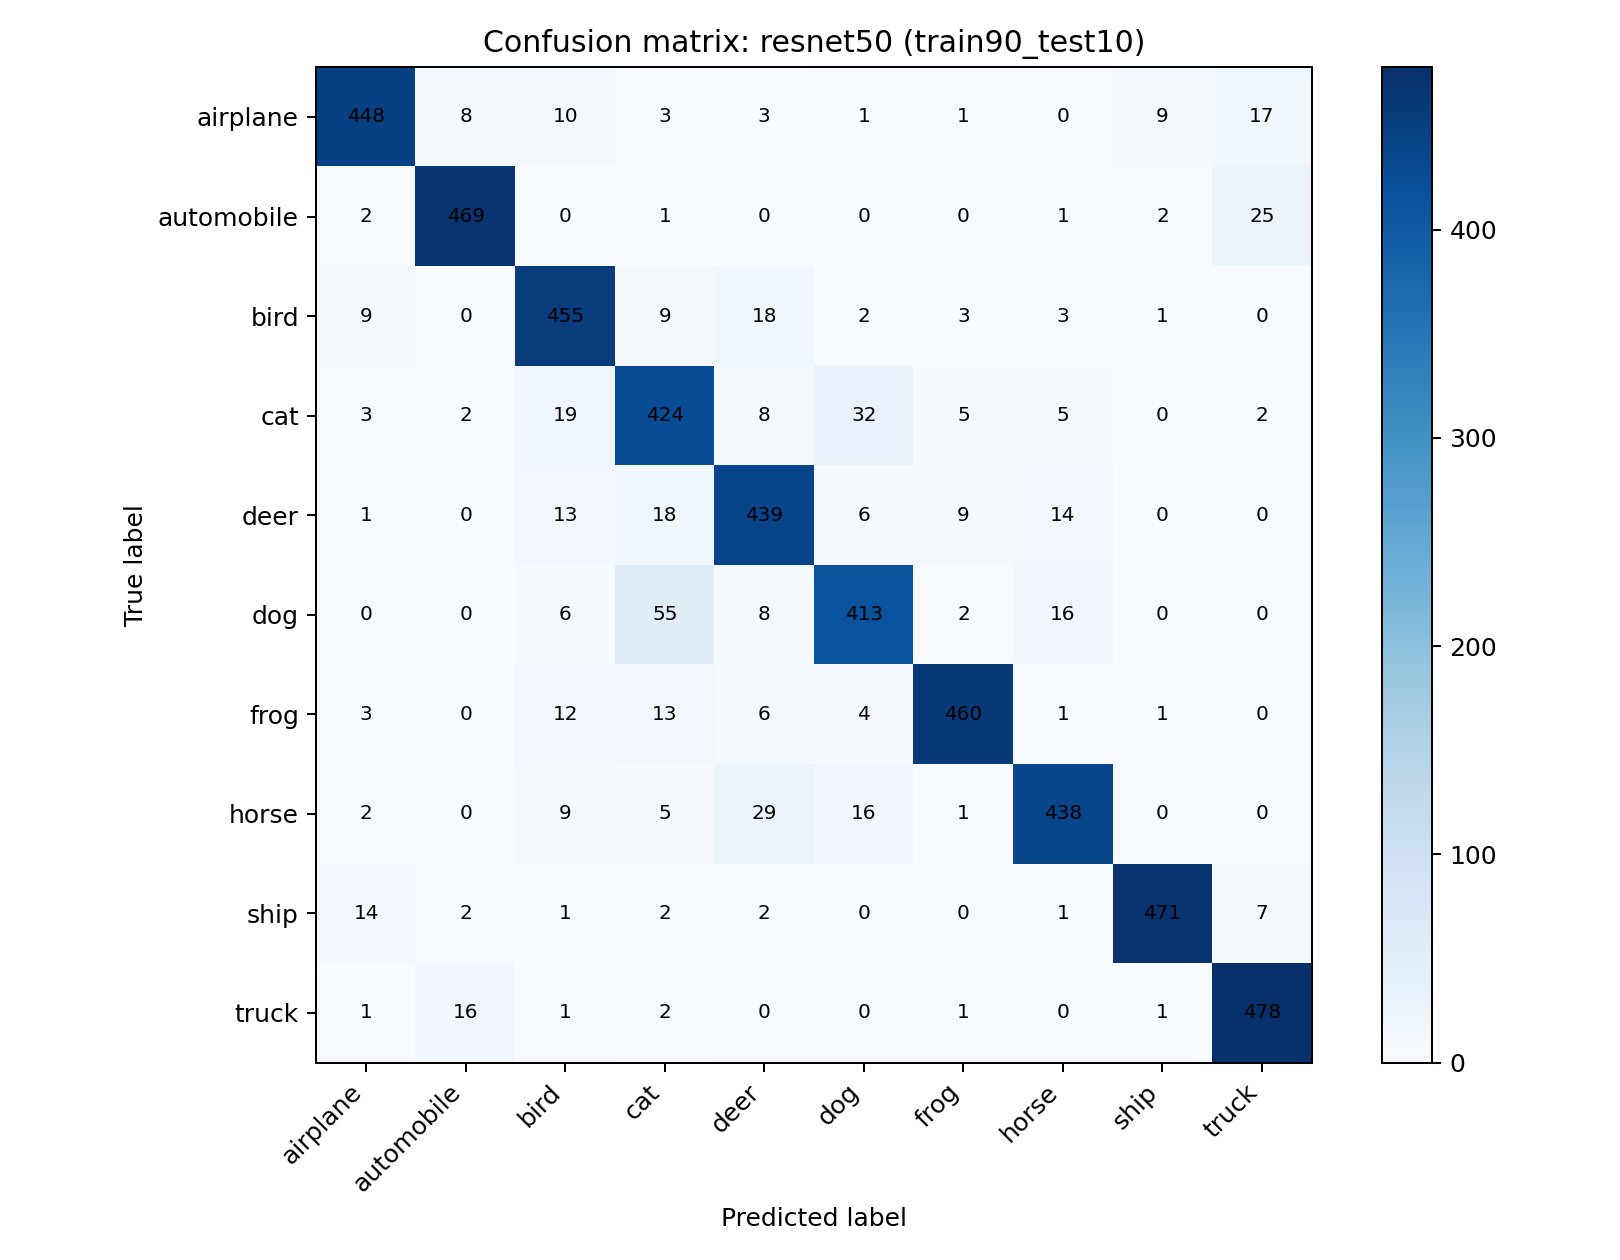
\includegraphics[width=0.75\textwidth]{../../outputs/split-impact-seed-42/plots/cm_resnet50_train90_test10.png}
    \caption{Macierz pomyłek dla najlepszej konfiguracji modelu ResNet50.}
    \label{fig:cm_res_best}
\end{figure}

\begin{figure}[H]
    \centering
    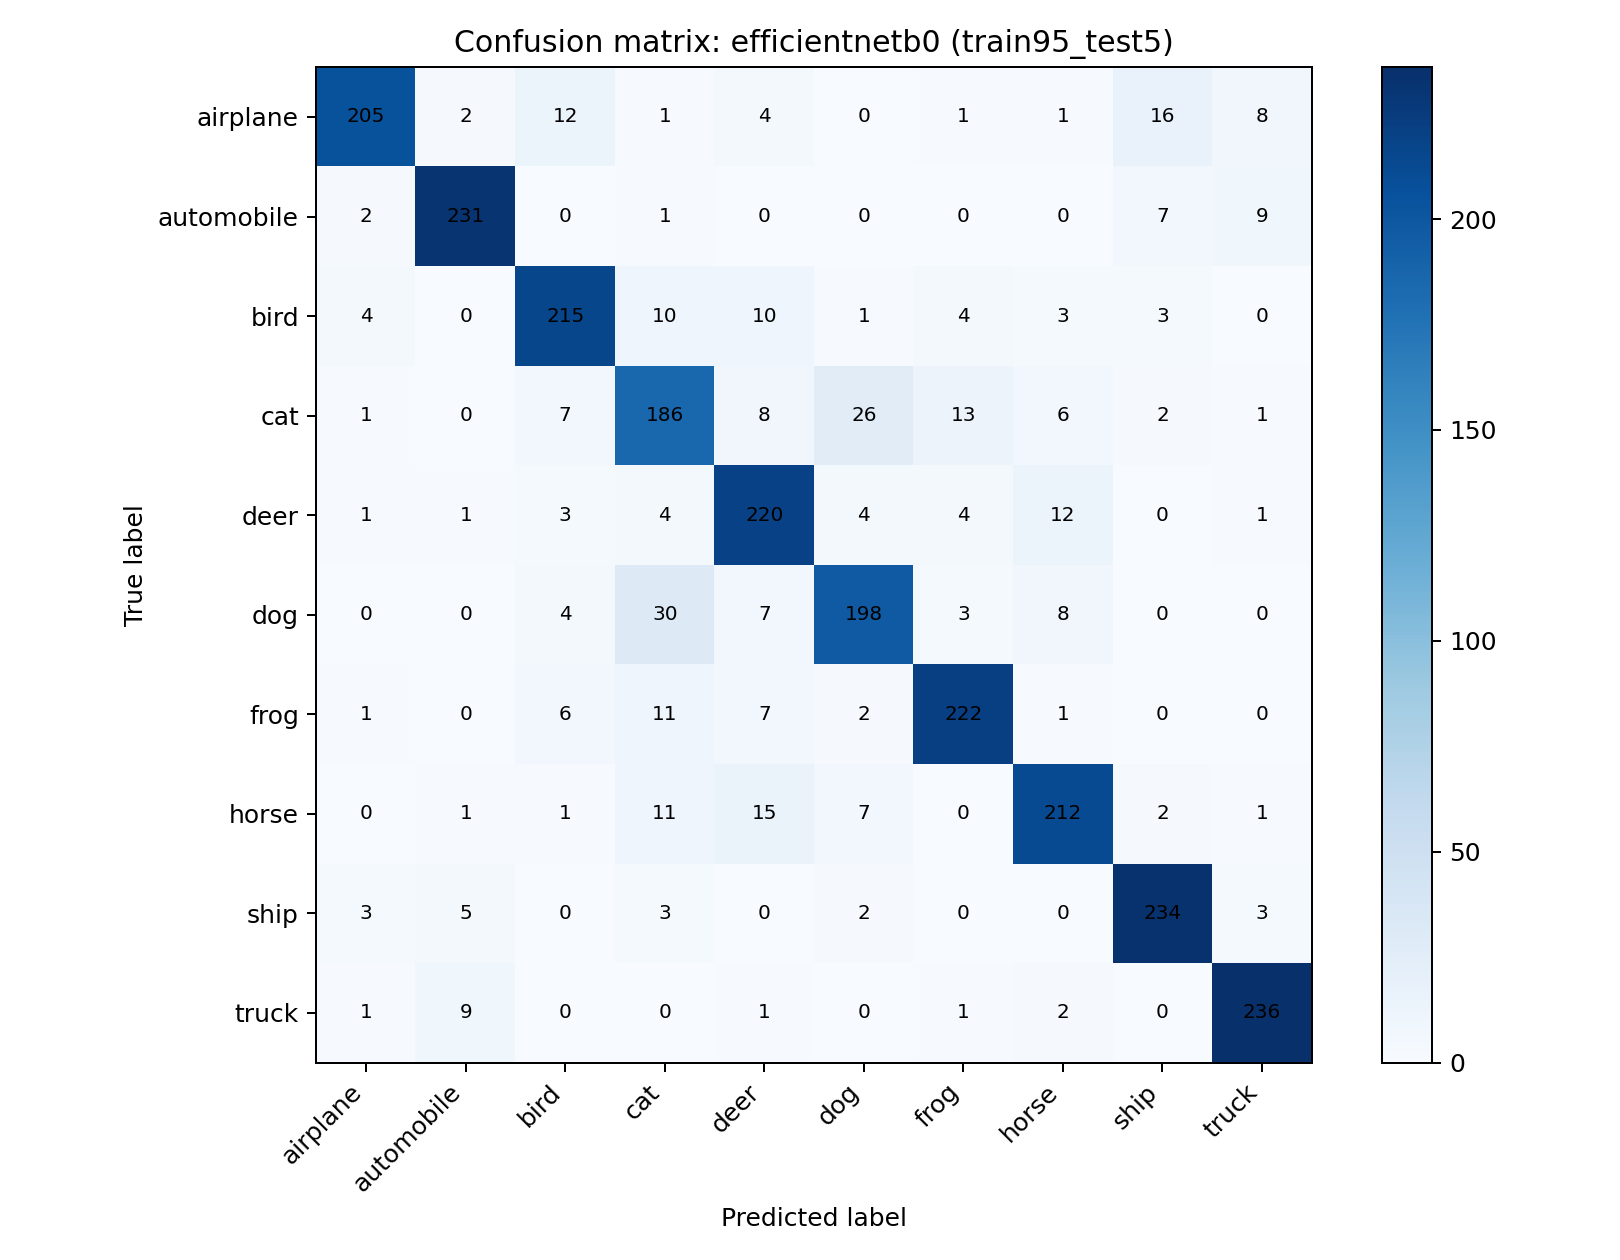
\includegraphics[width=0.75\textwidth]{../../outputs/split-impact-seed-42/plots/cm_efficientnetb0_train95_test5.png}
    \caption{Macierz pomyłek dla najlepszej konfiguracji modelu EfficientNetB0.}
    \label{fig:cm_eff_best}
\end{figure}

\begin{figure}[H]
    \centering
    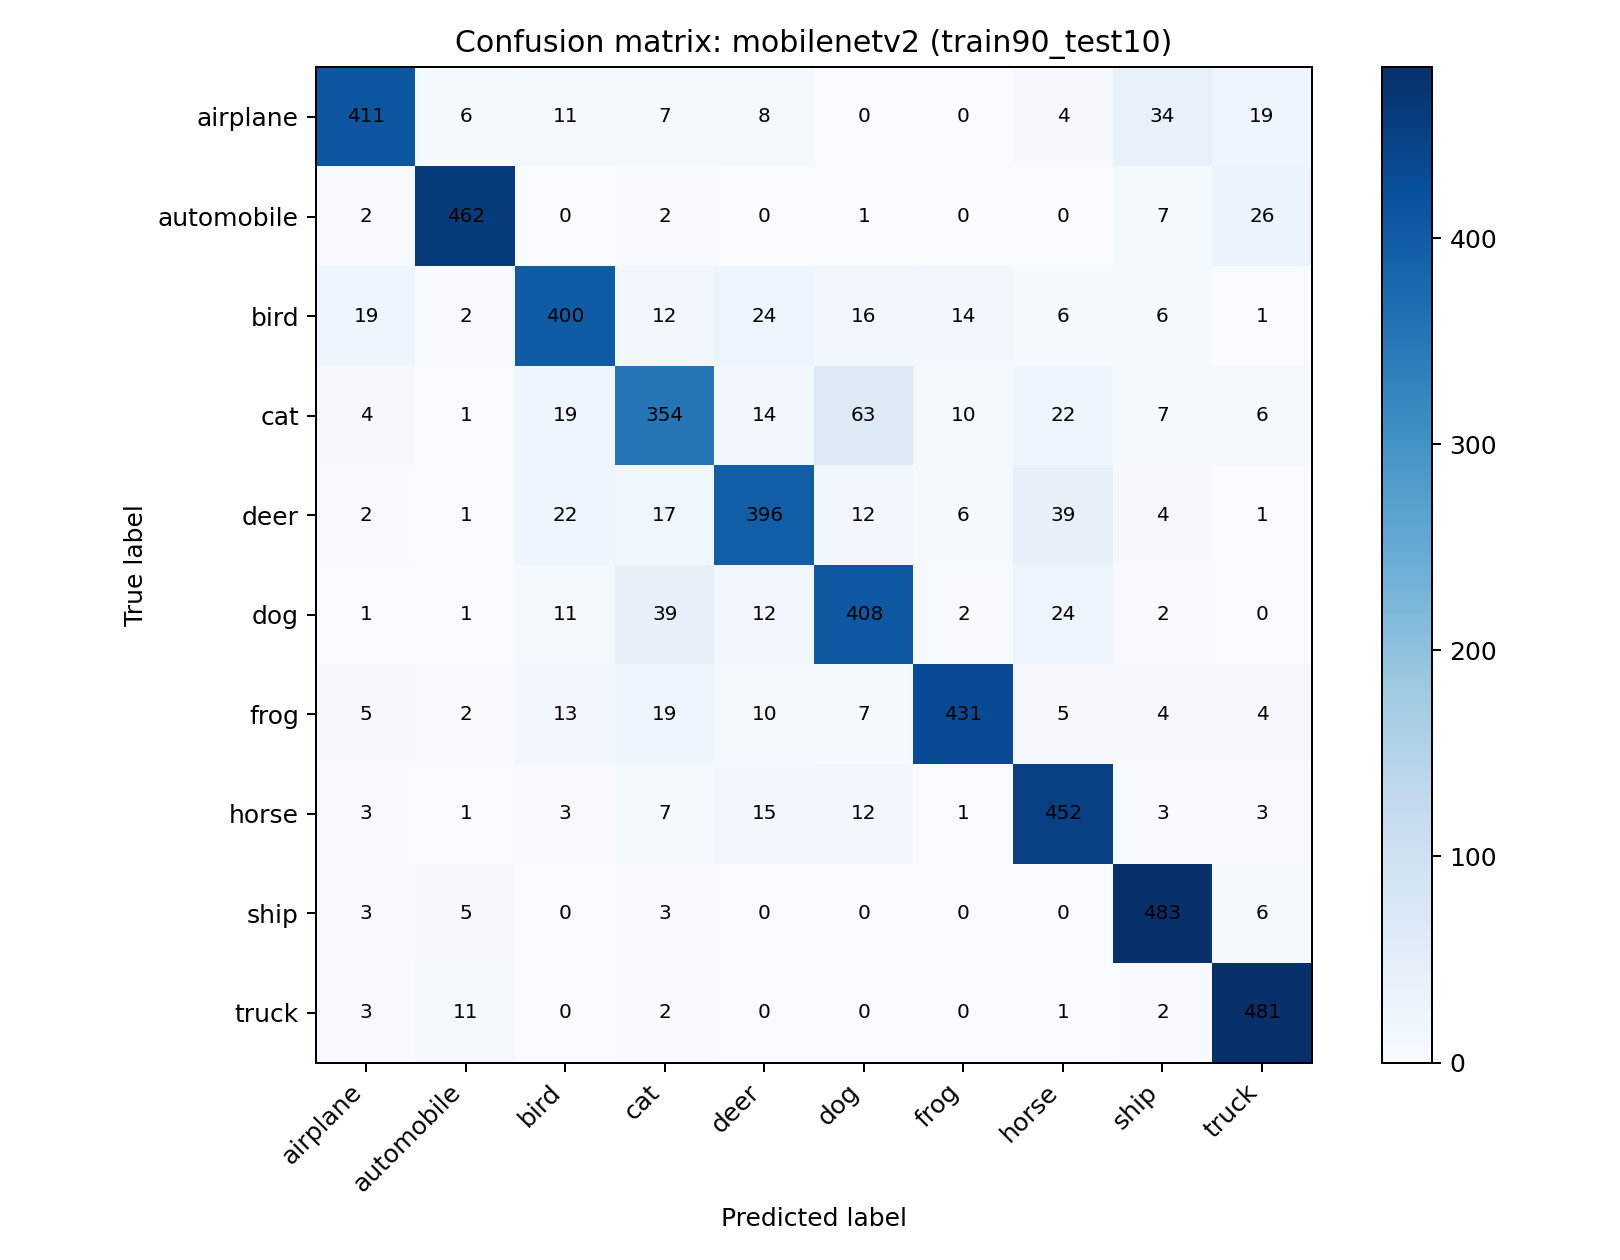
\includegraphics[width=0.75\textwidth]{../../outputs/split-impact-seed-42/plots/cm_mobilenetv2_train90_test10.png}
    \caption{Macierz pomyłek dla najlepszej konfiguracji modelu MobileNetV2.}
    \label{fig:cm_mob_best}
\end{figure}

% Opcjonalne wymuszenie nowej strony przed kolejną sekcją wykresów
\clearpage

% ============================================================
% NAJSŁABSZE KONFIGURACJE (Osobne figury)
% ============================================================

\begin{figure}[H]
    \centering
    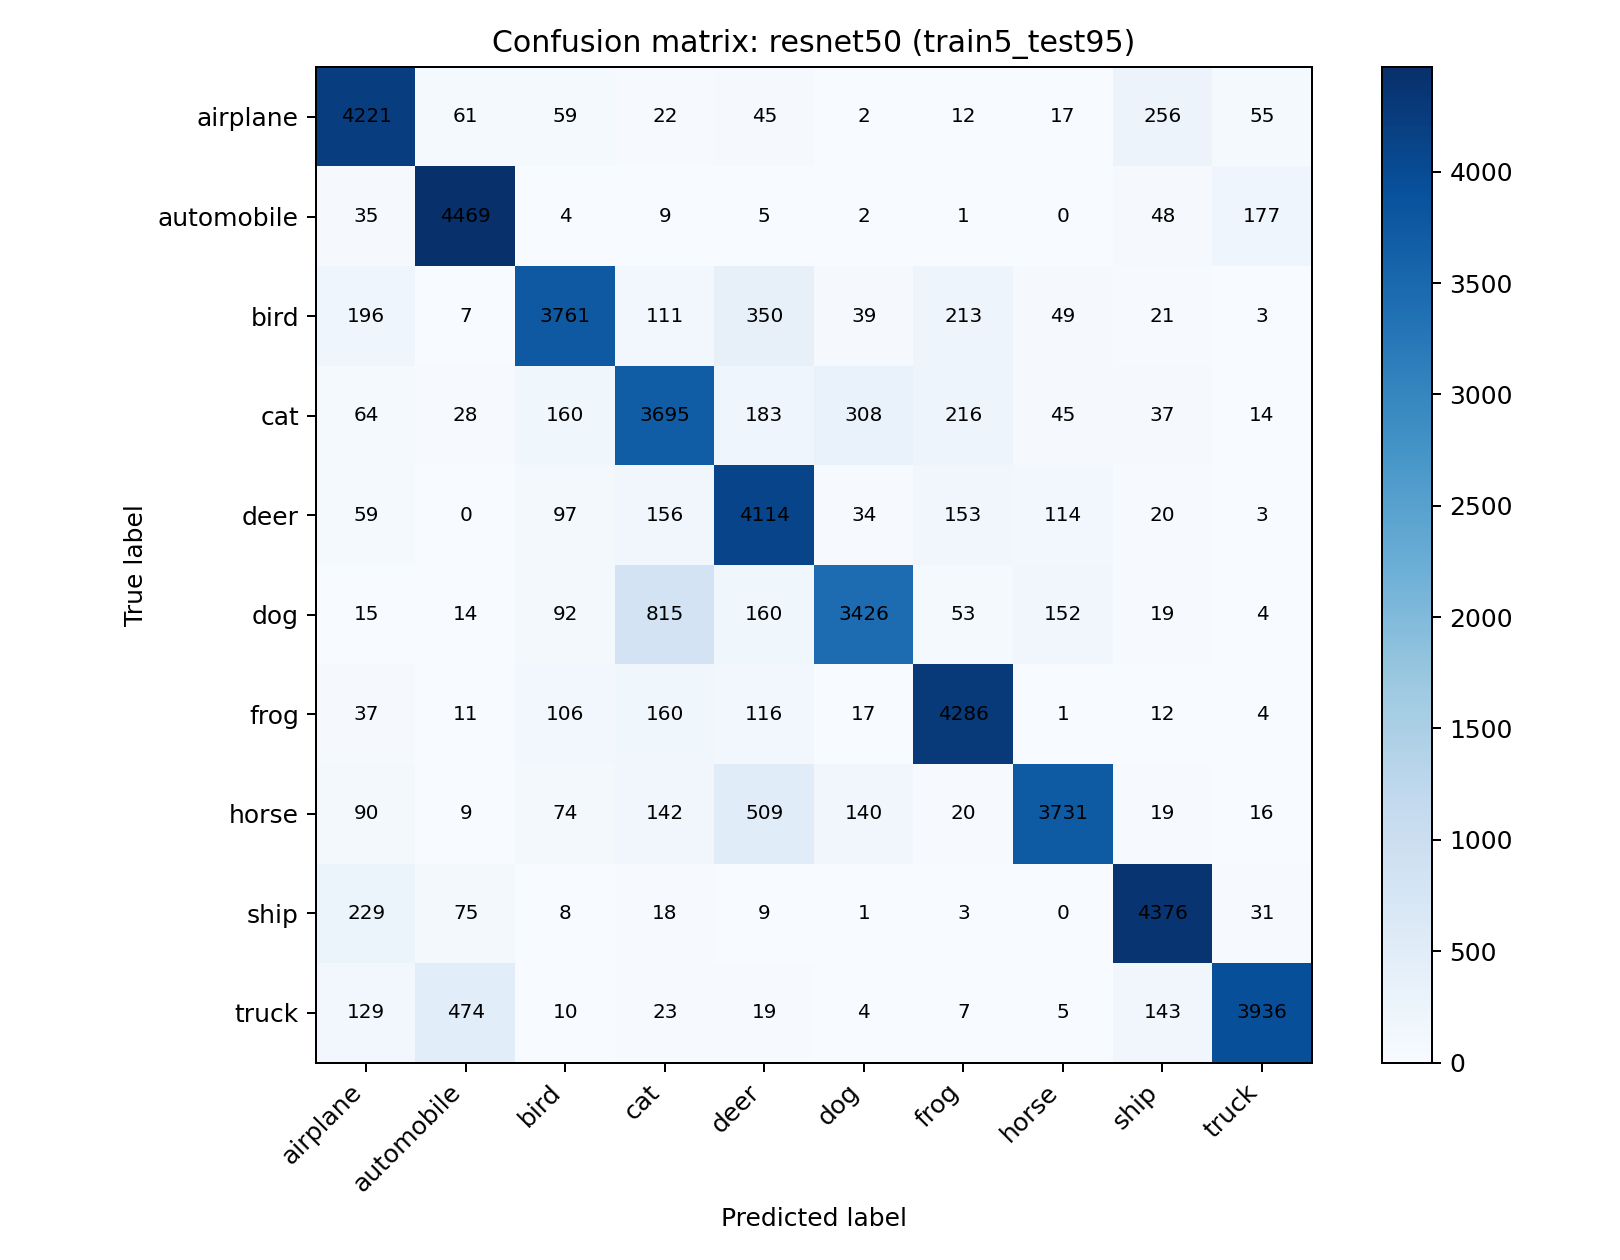
\includegraphics[width=0.75\textwidth]{../../outputs/split-impact-seed-42/plots/cm_resnet50_train5_test95.png}
    \caption{Macierz pomyłek dla najsłabszej konfiguracji modelu ResNet50.}
    \label{fig:cm_res_worst}
\end{figure}

\begin{figure}[H]
    \centering
    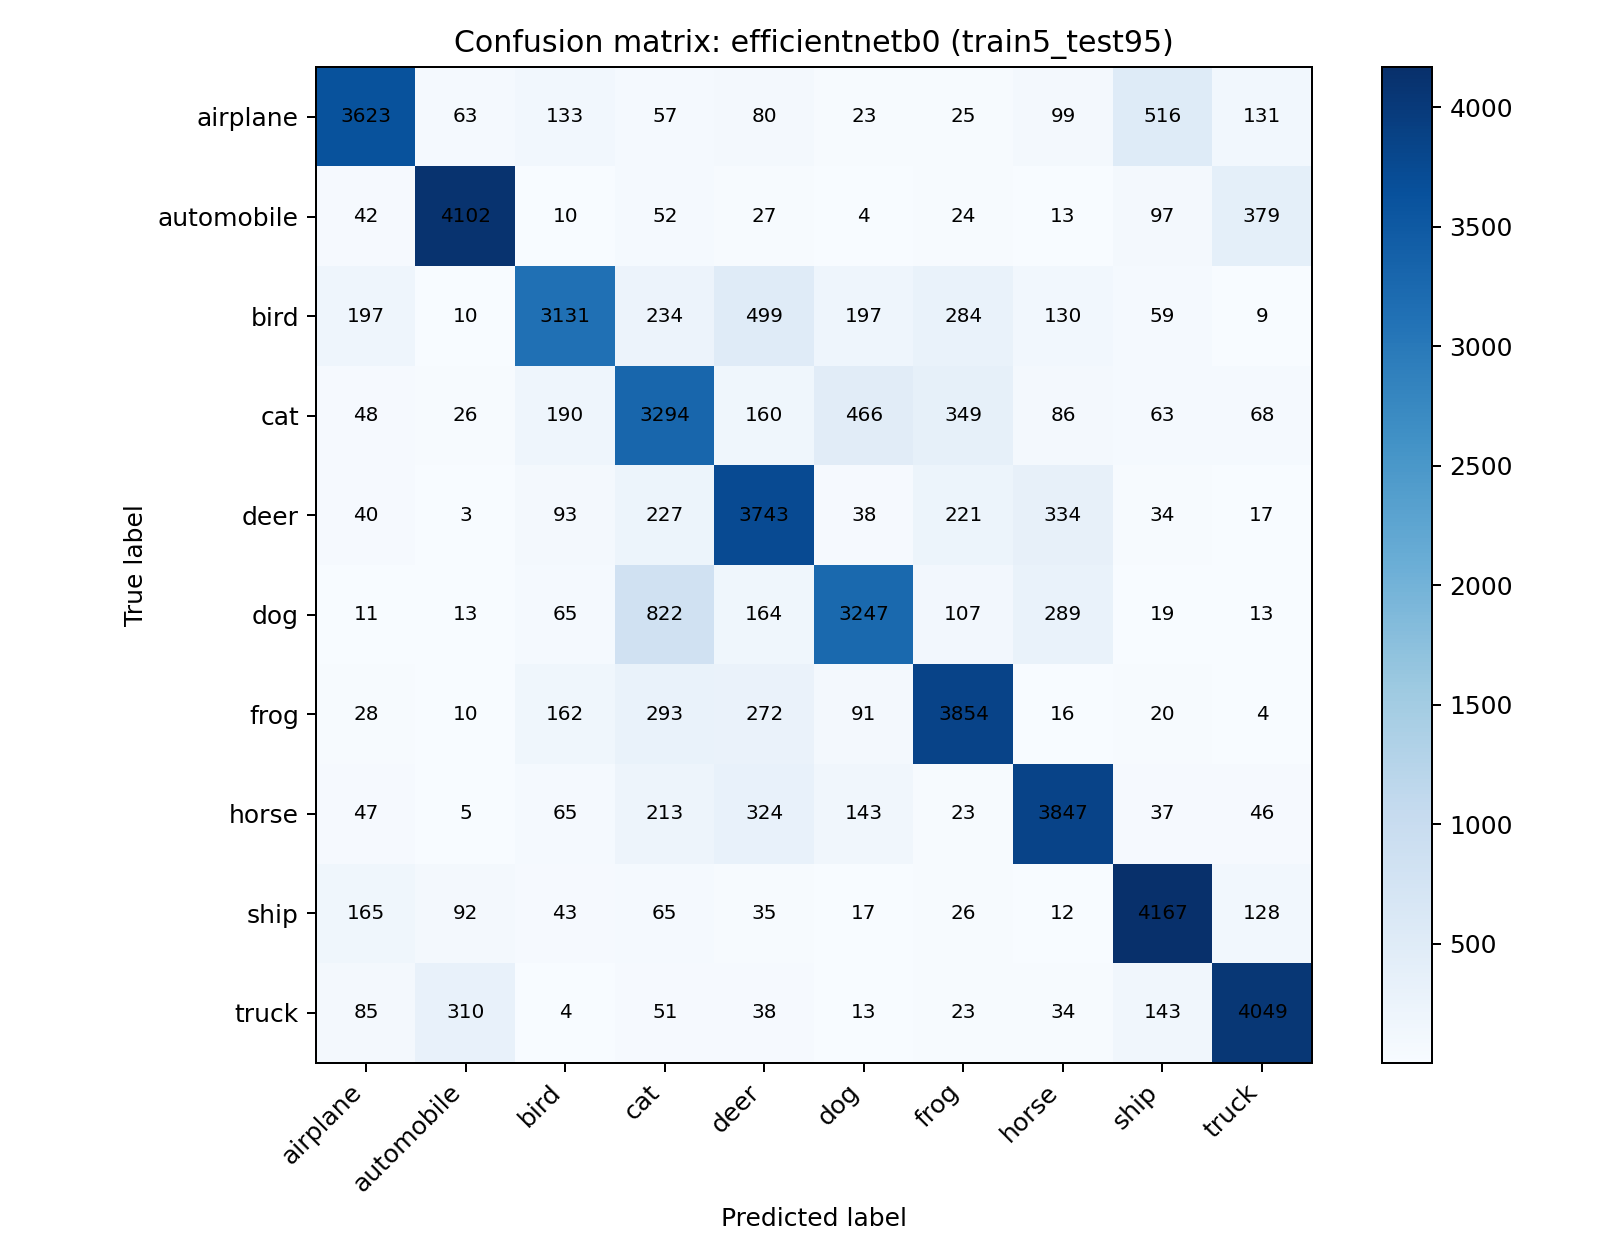
\includegraphics[width=0.75\textwidth]{../../outputs/split-impact-seed-42/plots/cm_efficientnetb0_train5_test95.png}
    \caption{Macierz pomyłek dla najsłabszej konfiguracji modelu EfficientNetB0.}
    \label{fig:cm_eff_worst}
\end{figure}

\begin{figure}[H]
    \centering
    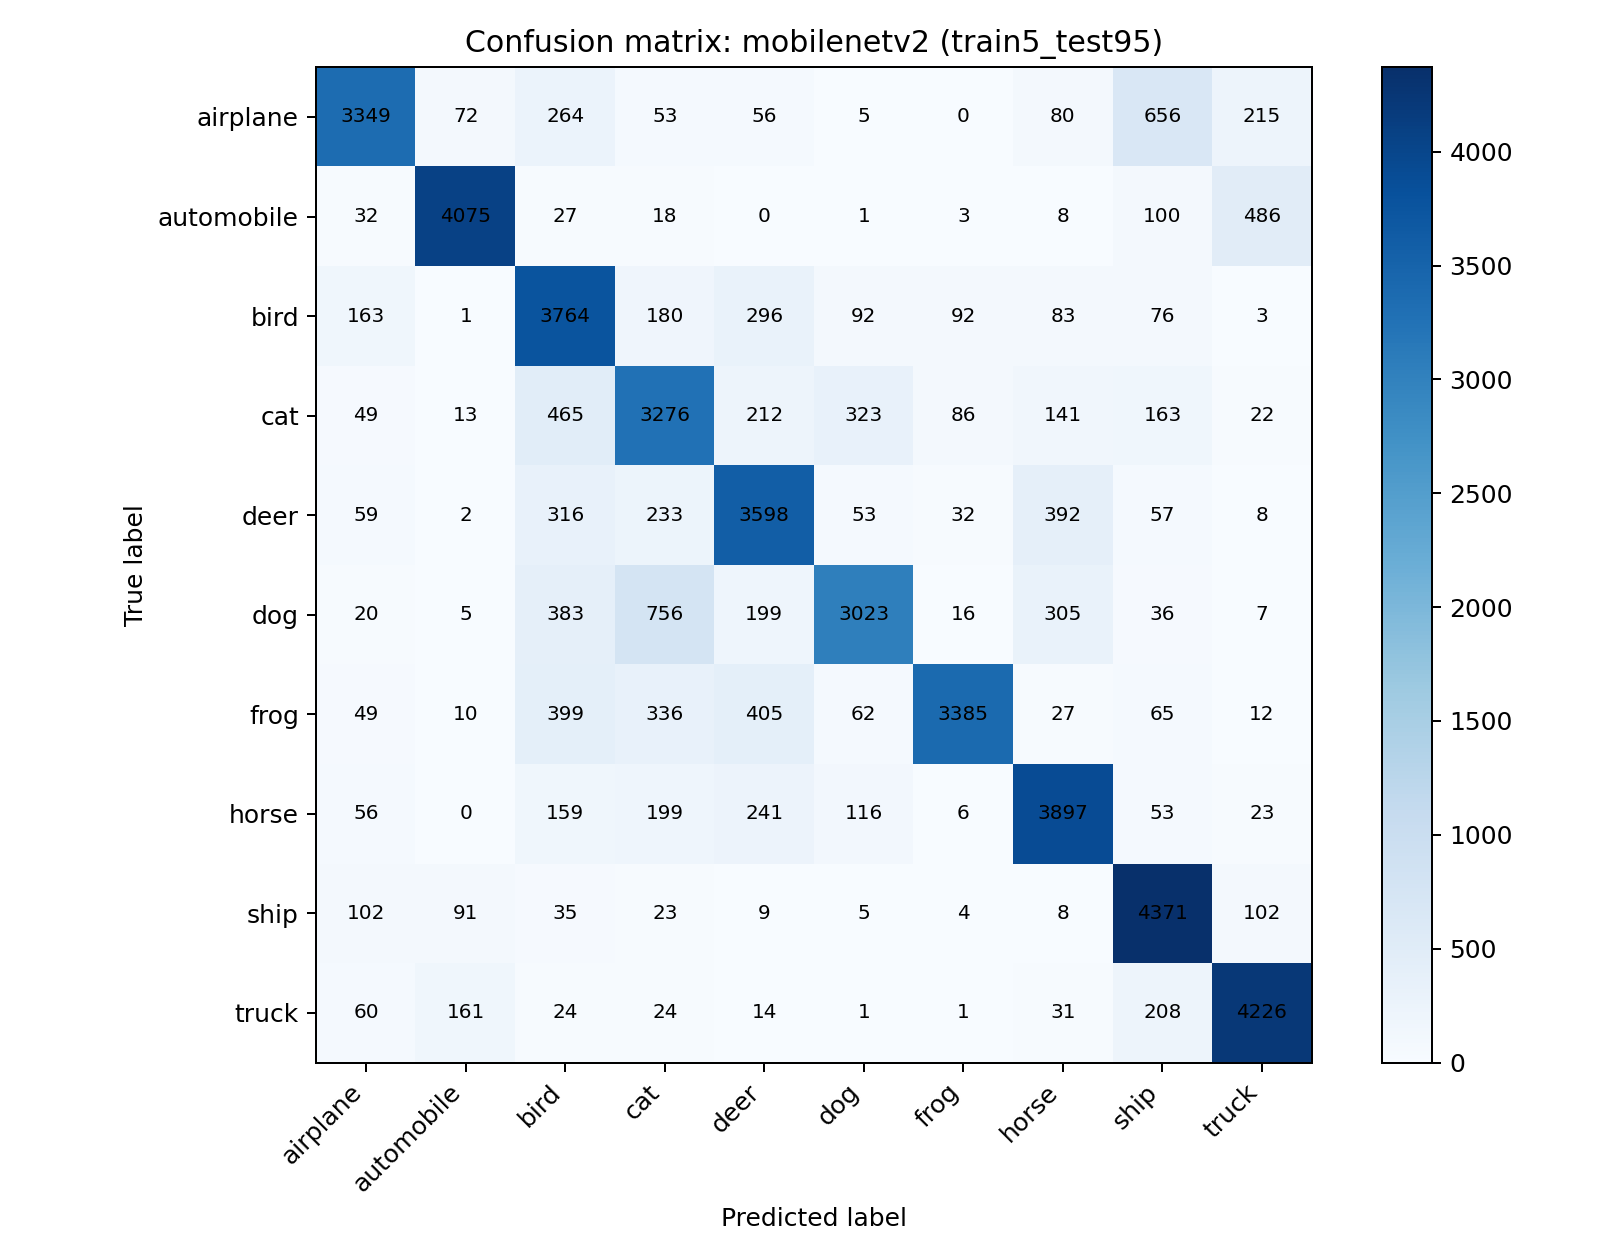
\includegraphics[width=0.75\textwidth]{../../outputs/split-impact-seed-42/plots/cm_mobilenetv2_train5_test95.png}
    \caption{Macierz pomyłek dla najsłabszej konfiguracji modelu MobileNetV2.}
    \label{fig:cm_mob_worst}
\end{figure}
\subsection{Analiza krzywych ROC i wartości AUC}

Istotnym kryterium oceny modeli wieloklasowych jest charakterystyka krzywej ROC (ang. \textit{Receiver Operating Characteristic}) oraz pole pod tą krzywą (AUC). Obliczenia przeprowadzono z wykorzystaniem podejścia Macro OVR (\textit{One-vs-Rest}) uśredniającego wagę każdej z klas w równym stopniu, oraz podejścia Micro, agregującego globalnie wkłady wszystkich próbek. 

Jak wykazano w tabeli \ref{tab:best_results}, architektura ResNet50 w optymalnej konfiguracji osiągnęła wynik $\text{ROC AUC}_{\text{Macro}} = 0.9943$, co wskazuje na niemal perfekcyjną zdolność do separacji klas. 

W celu zobrazowania wpływu rozmiaru zbioru treningowego na pewność predykcji, na rysunku \ref{fig:roc_curves_combined} zestawiono optymalne krzywe ROC dla wszystkich trzech badanych architektur oraz, dla kontrastu, krzywą uzyskaną przez model ResNet50 trenowany na zaledwie 5\% danych.

\begin{figure}[H]
    \centering
    % Górny wiersz: ResNet50 (Najlepszy vs Najgorszy)
    \begin{subfigure}{0.48\textwidth}
        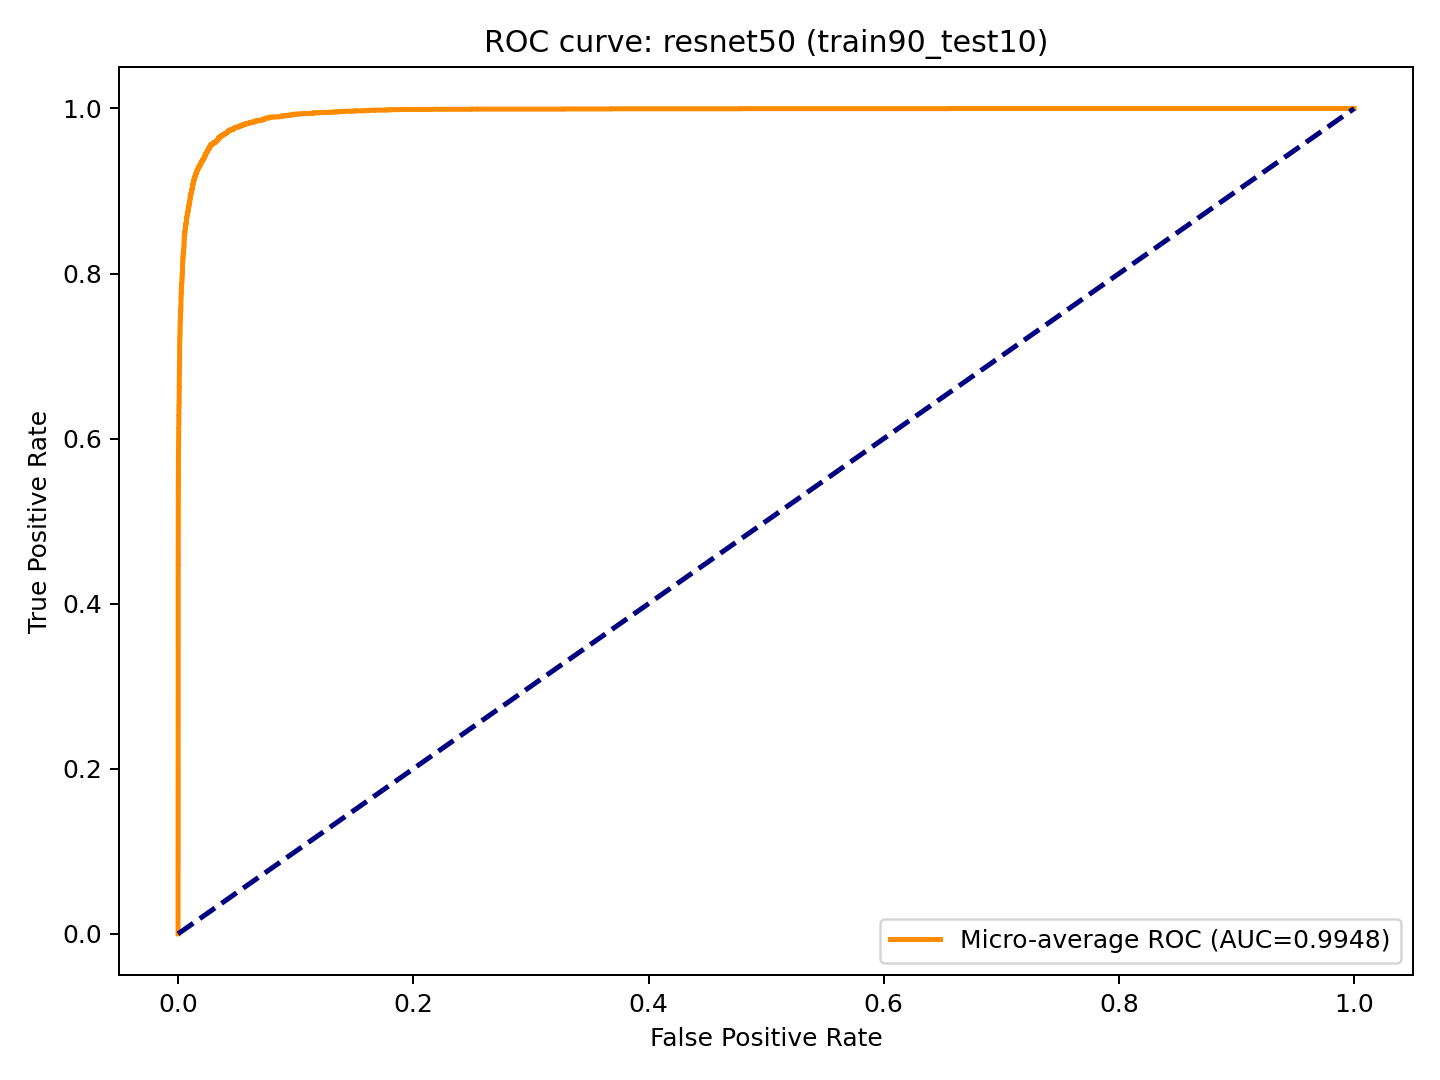
\includegraphics[width=\linewidth]{../../outputs/split-impact-seed-42/plots/roc_resnet50_train90_test10.png}
        \caption{ResNet50 (Najlepszy: train90\_test10)}
        \label{fig:roc_res_best}
    \end{subfigure}
    \hfill
    \begin{subfigure}{0.48\textwidth}
        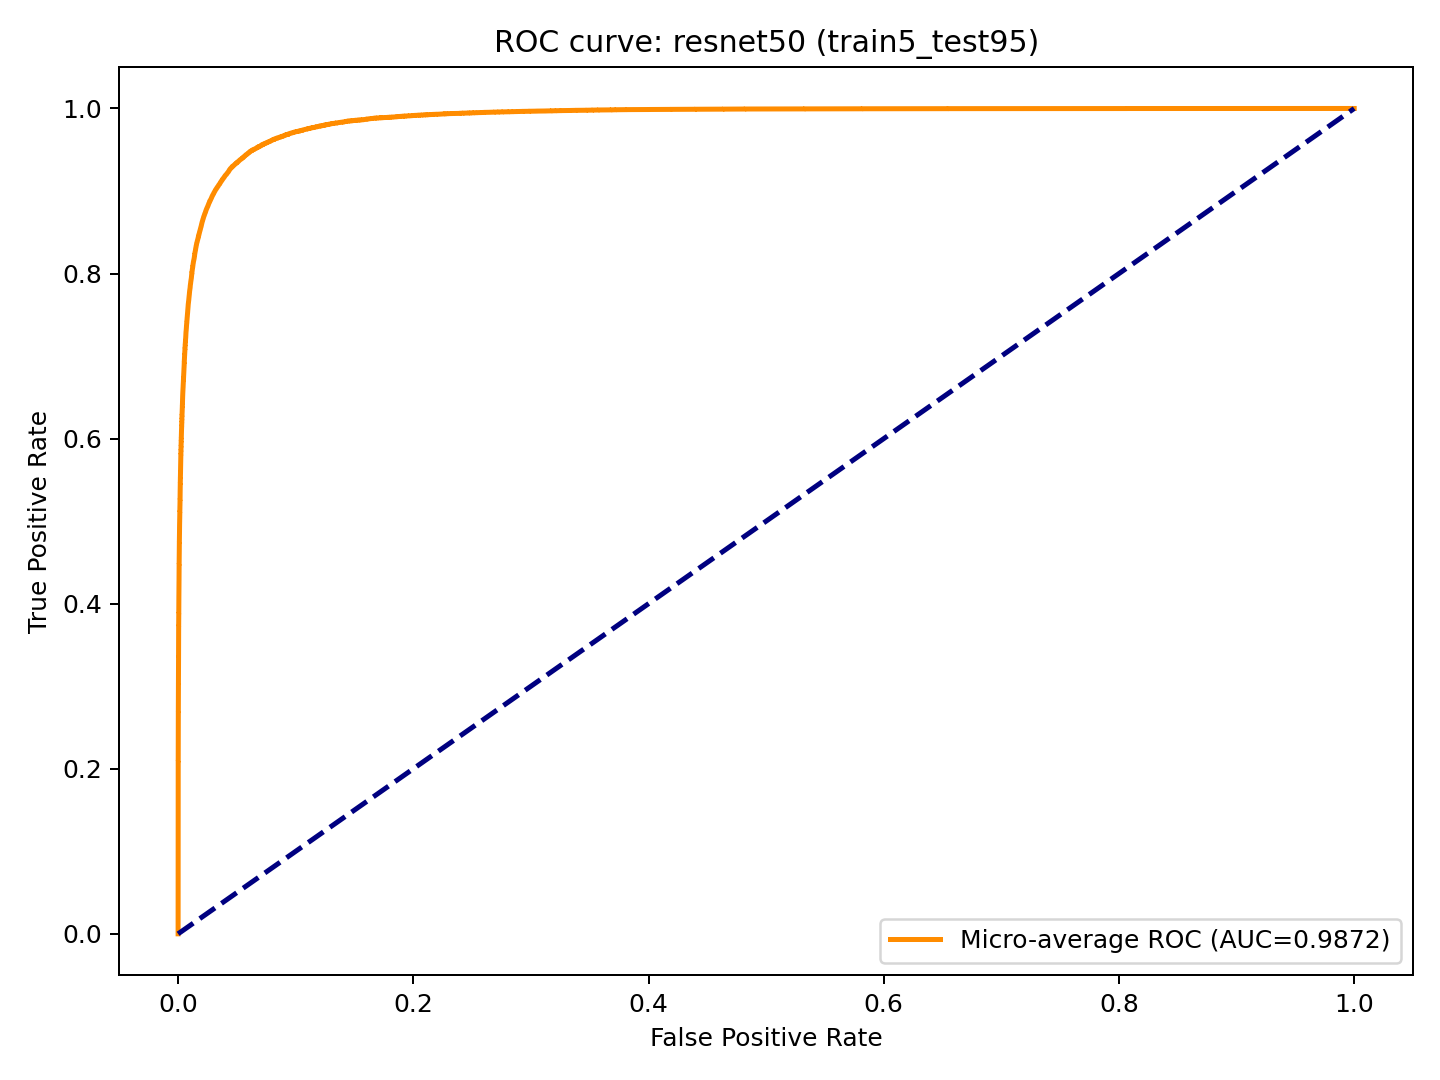
\includegraphics[width=\linewidth]{../../outputs/split-impact-seed-42/plots/roc_resnet50_train5_test95.png}
        \caption{ResNet50 (Najsłabszy: train5\_test95)}
        \label{fig:roc_res_worst}
    \end{subfigure}
    
    \vspace{0.4cm}
    % Dolny wiersz: Najlepsze warianty pozostałych modeli
    \begin{subfigure}{0.48\textwidth}
        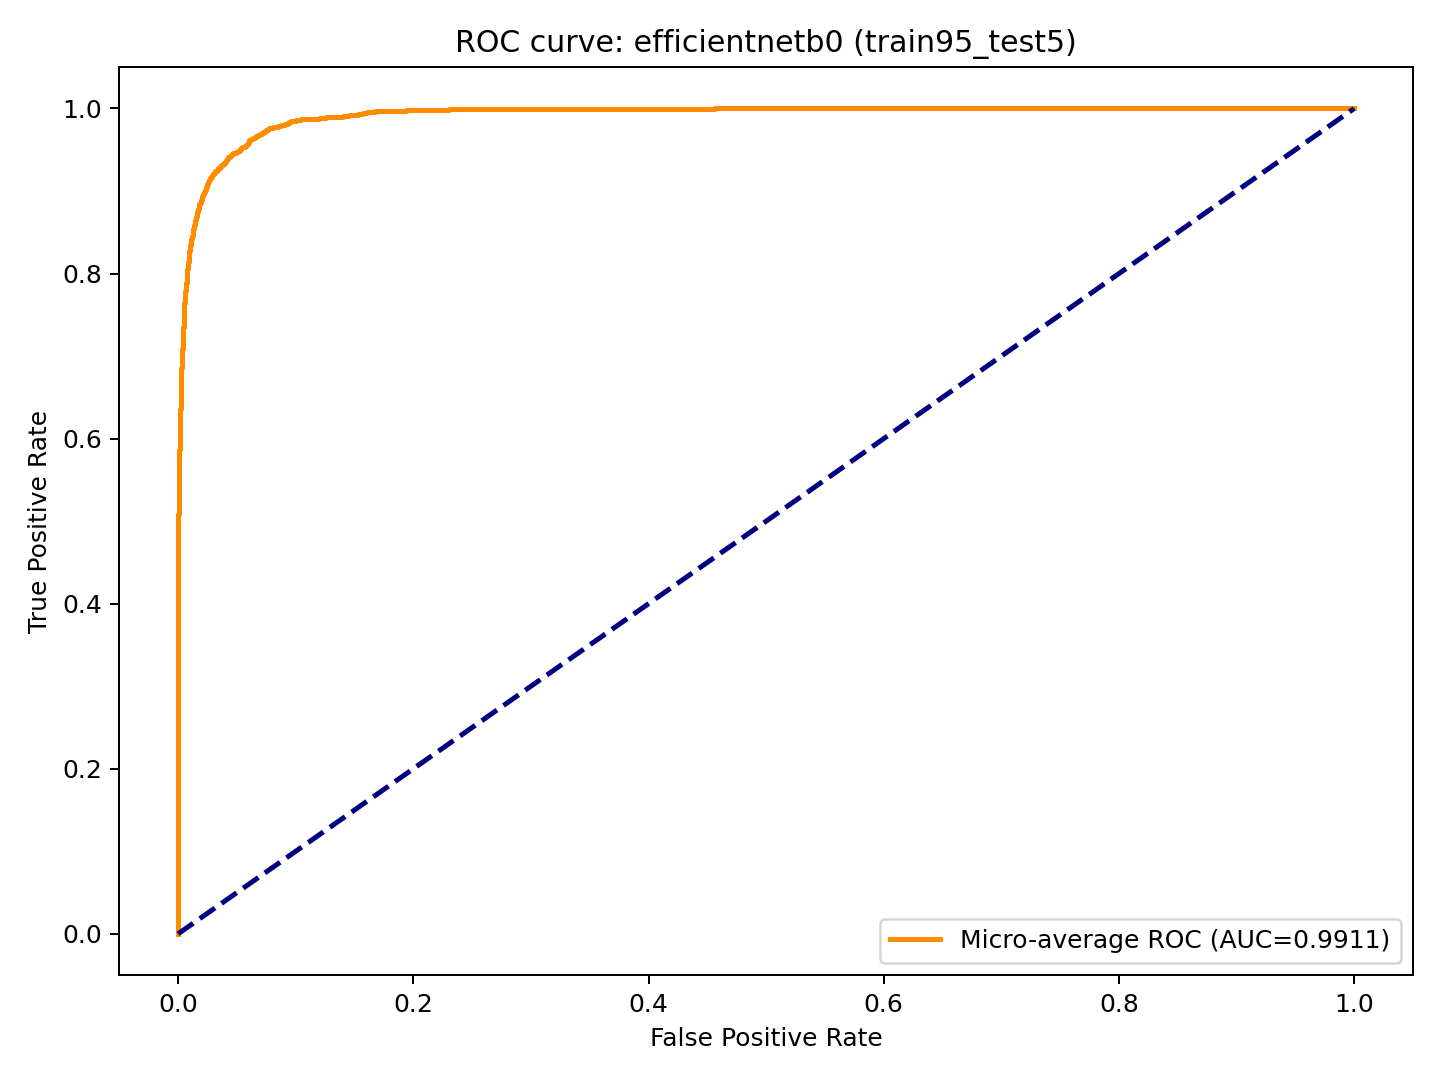
\includegraphics[width=\linewidth]{../../outputs/split-impact-seed-42/plots/roc_efficientnetb0_train95_test5.png}
        \caption{EfficientNetB0 (Najlepszy: train95\_test5)}
        \label{fig:roc_eff_best}
    \end{subfigure}
    \hfill
    \begin{subfigure}{0.48\textwidth}
        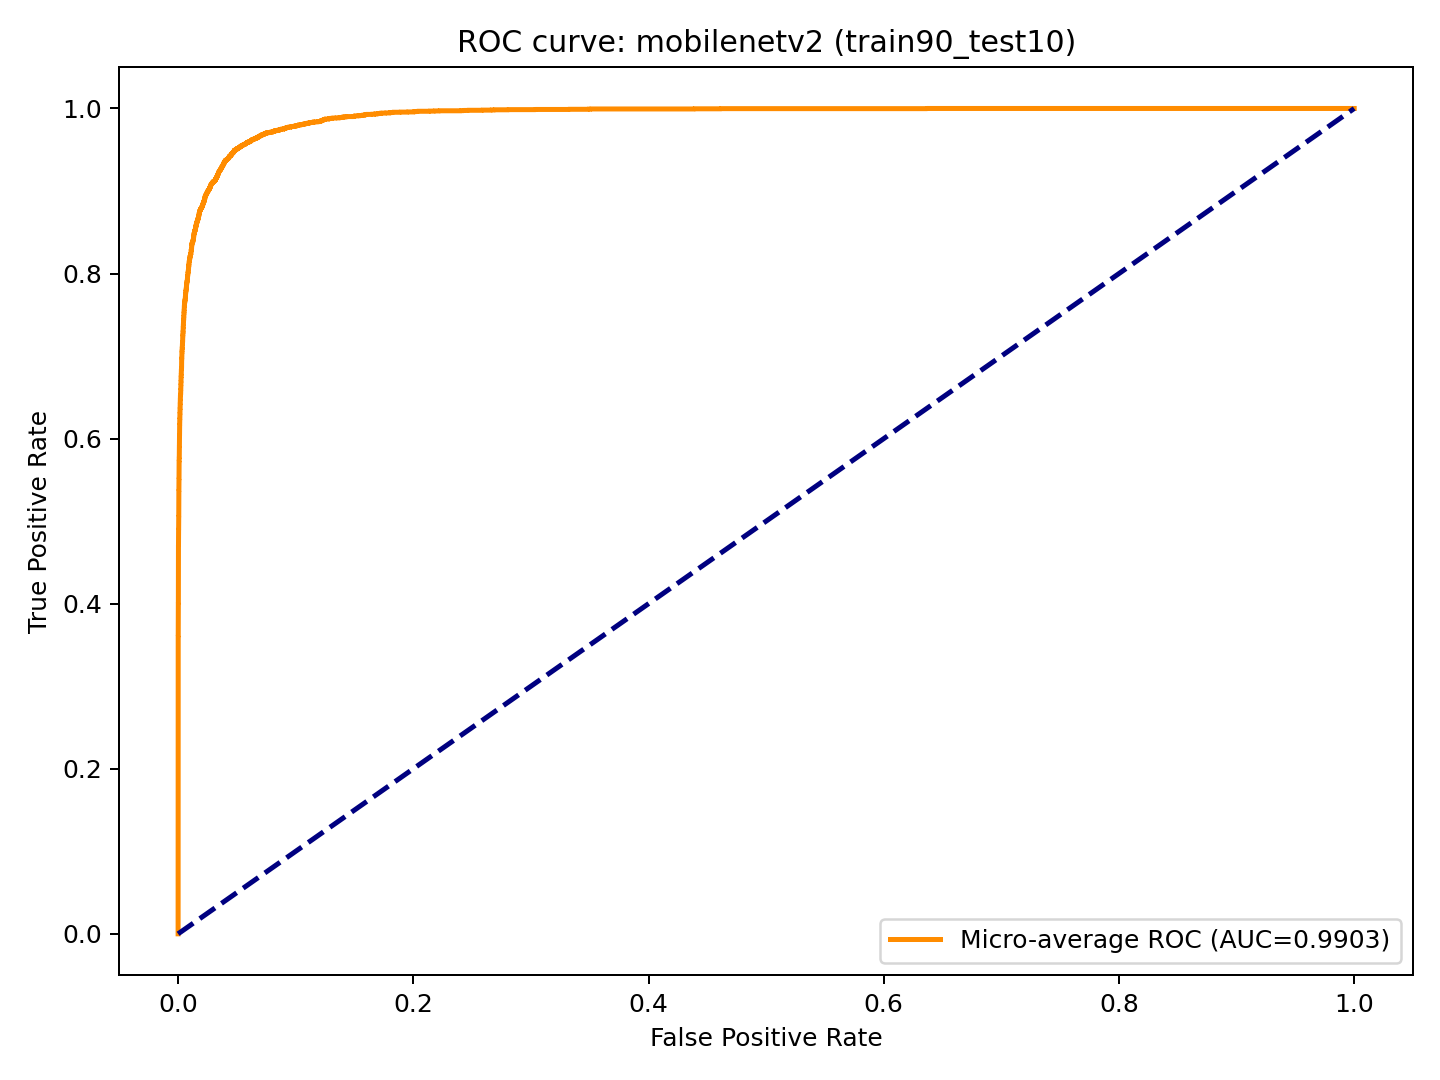
\includegraphics[width=\linewidth]{../../outputs/split-impact-seed-42/plots/roc_mobilenetv2_train90_test10.png}
        \caption{MobileNetV2 (Najlepszy: train90\_test10)}
        \label{fig:roc_mob_best}
    \end{subfigure}
    
    \caption{Zestawienie krzywych ROC oraz wartości AUC dla optymalnych konfiguracji badanych modeli oraz wariantu ze skrajnie ograniczonym zbiorem treningowym.}
    \label{fig:roc_curves_combined}
\end{figure}


\subsection{Wizualizacja predykcji dla najlepszych konfiguracji}

Dla zobrazowania praktycznego działania wyuczonych sieci, na poniższych rysunkach przedstawiono przykładowe predykcje obrazów ze zbioru testowego dla najlepszych konfiguracji każdego z badanych modeli. Na każdy kafelek nałożono etykietę rzeczywistą (T: \textit{True}) oraz etykietę przewidywaną przez model (P: \textit{Predicted}). Kolorem zielonym oznaczono poprawne klasyfikacje, natomiast kolorem czerwonym przypadki błędne.

% ============================================================
% PREDYKCJE - RESNET50
% ============================================================
\begin{figure}[H]
    \centering
    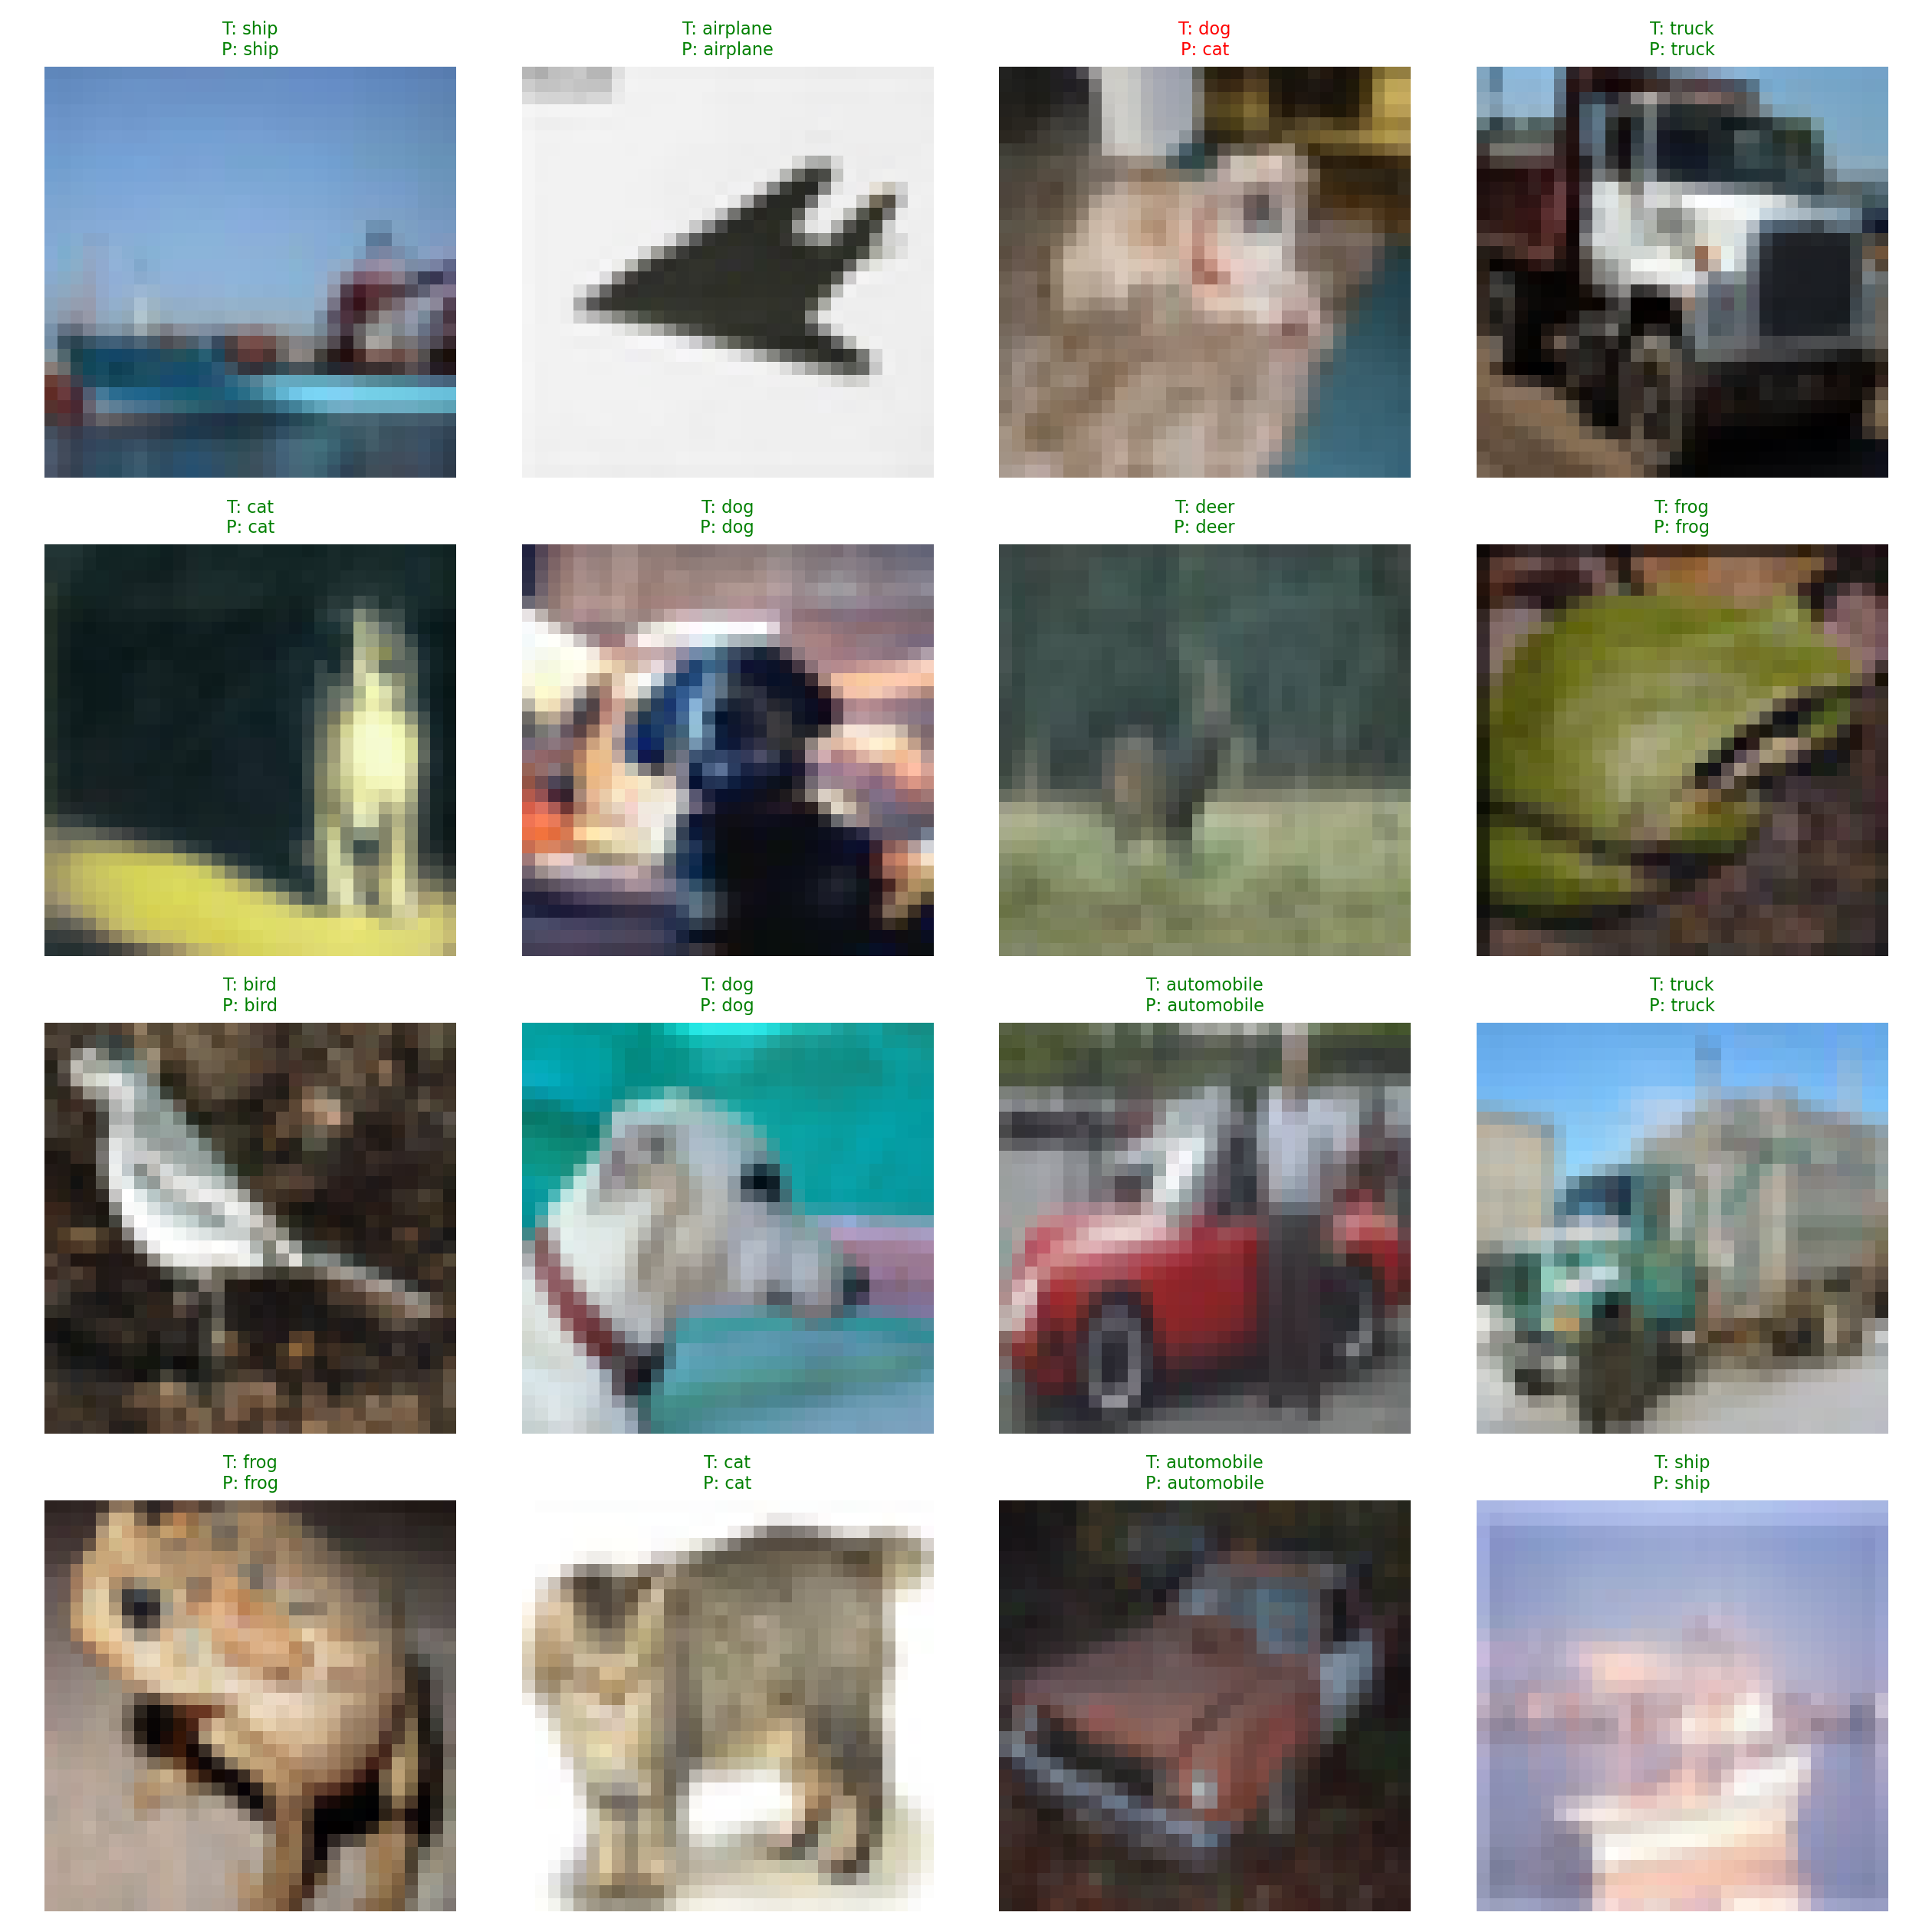
\includegraphics[width=0.85\textwidth]{../../outputs/split-impact-seed-42/plots/predictions_resnet50_train90_test10.png}
    \caption{Przykładowa siatka predykcji dla najlepszej konfiguracji modelu \textbf{ResNet50} (wariant train90\_test10).}
    \label{fig:predictions_resnet_best}
\end{figure}

% ============================================================
% PREDYKCJE - EFFICIENTNETB0
% ============================================================
\begin{figure}[H]
    \centering
    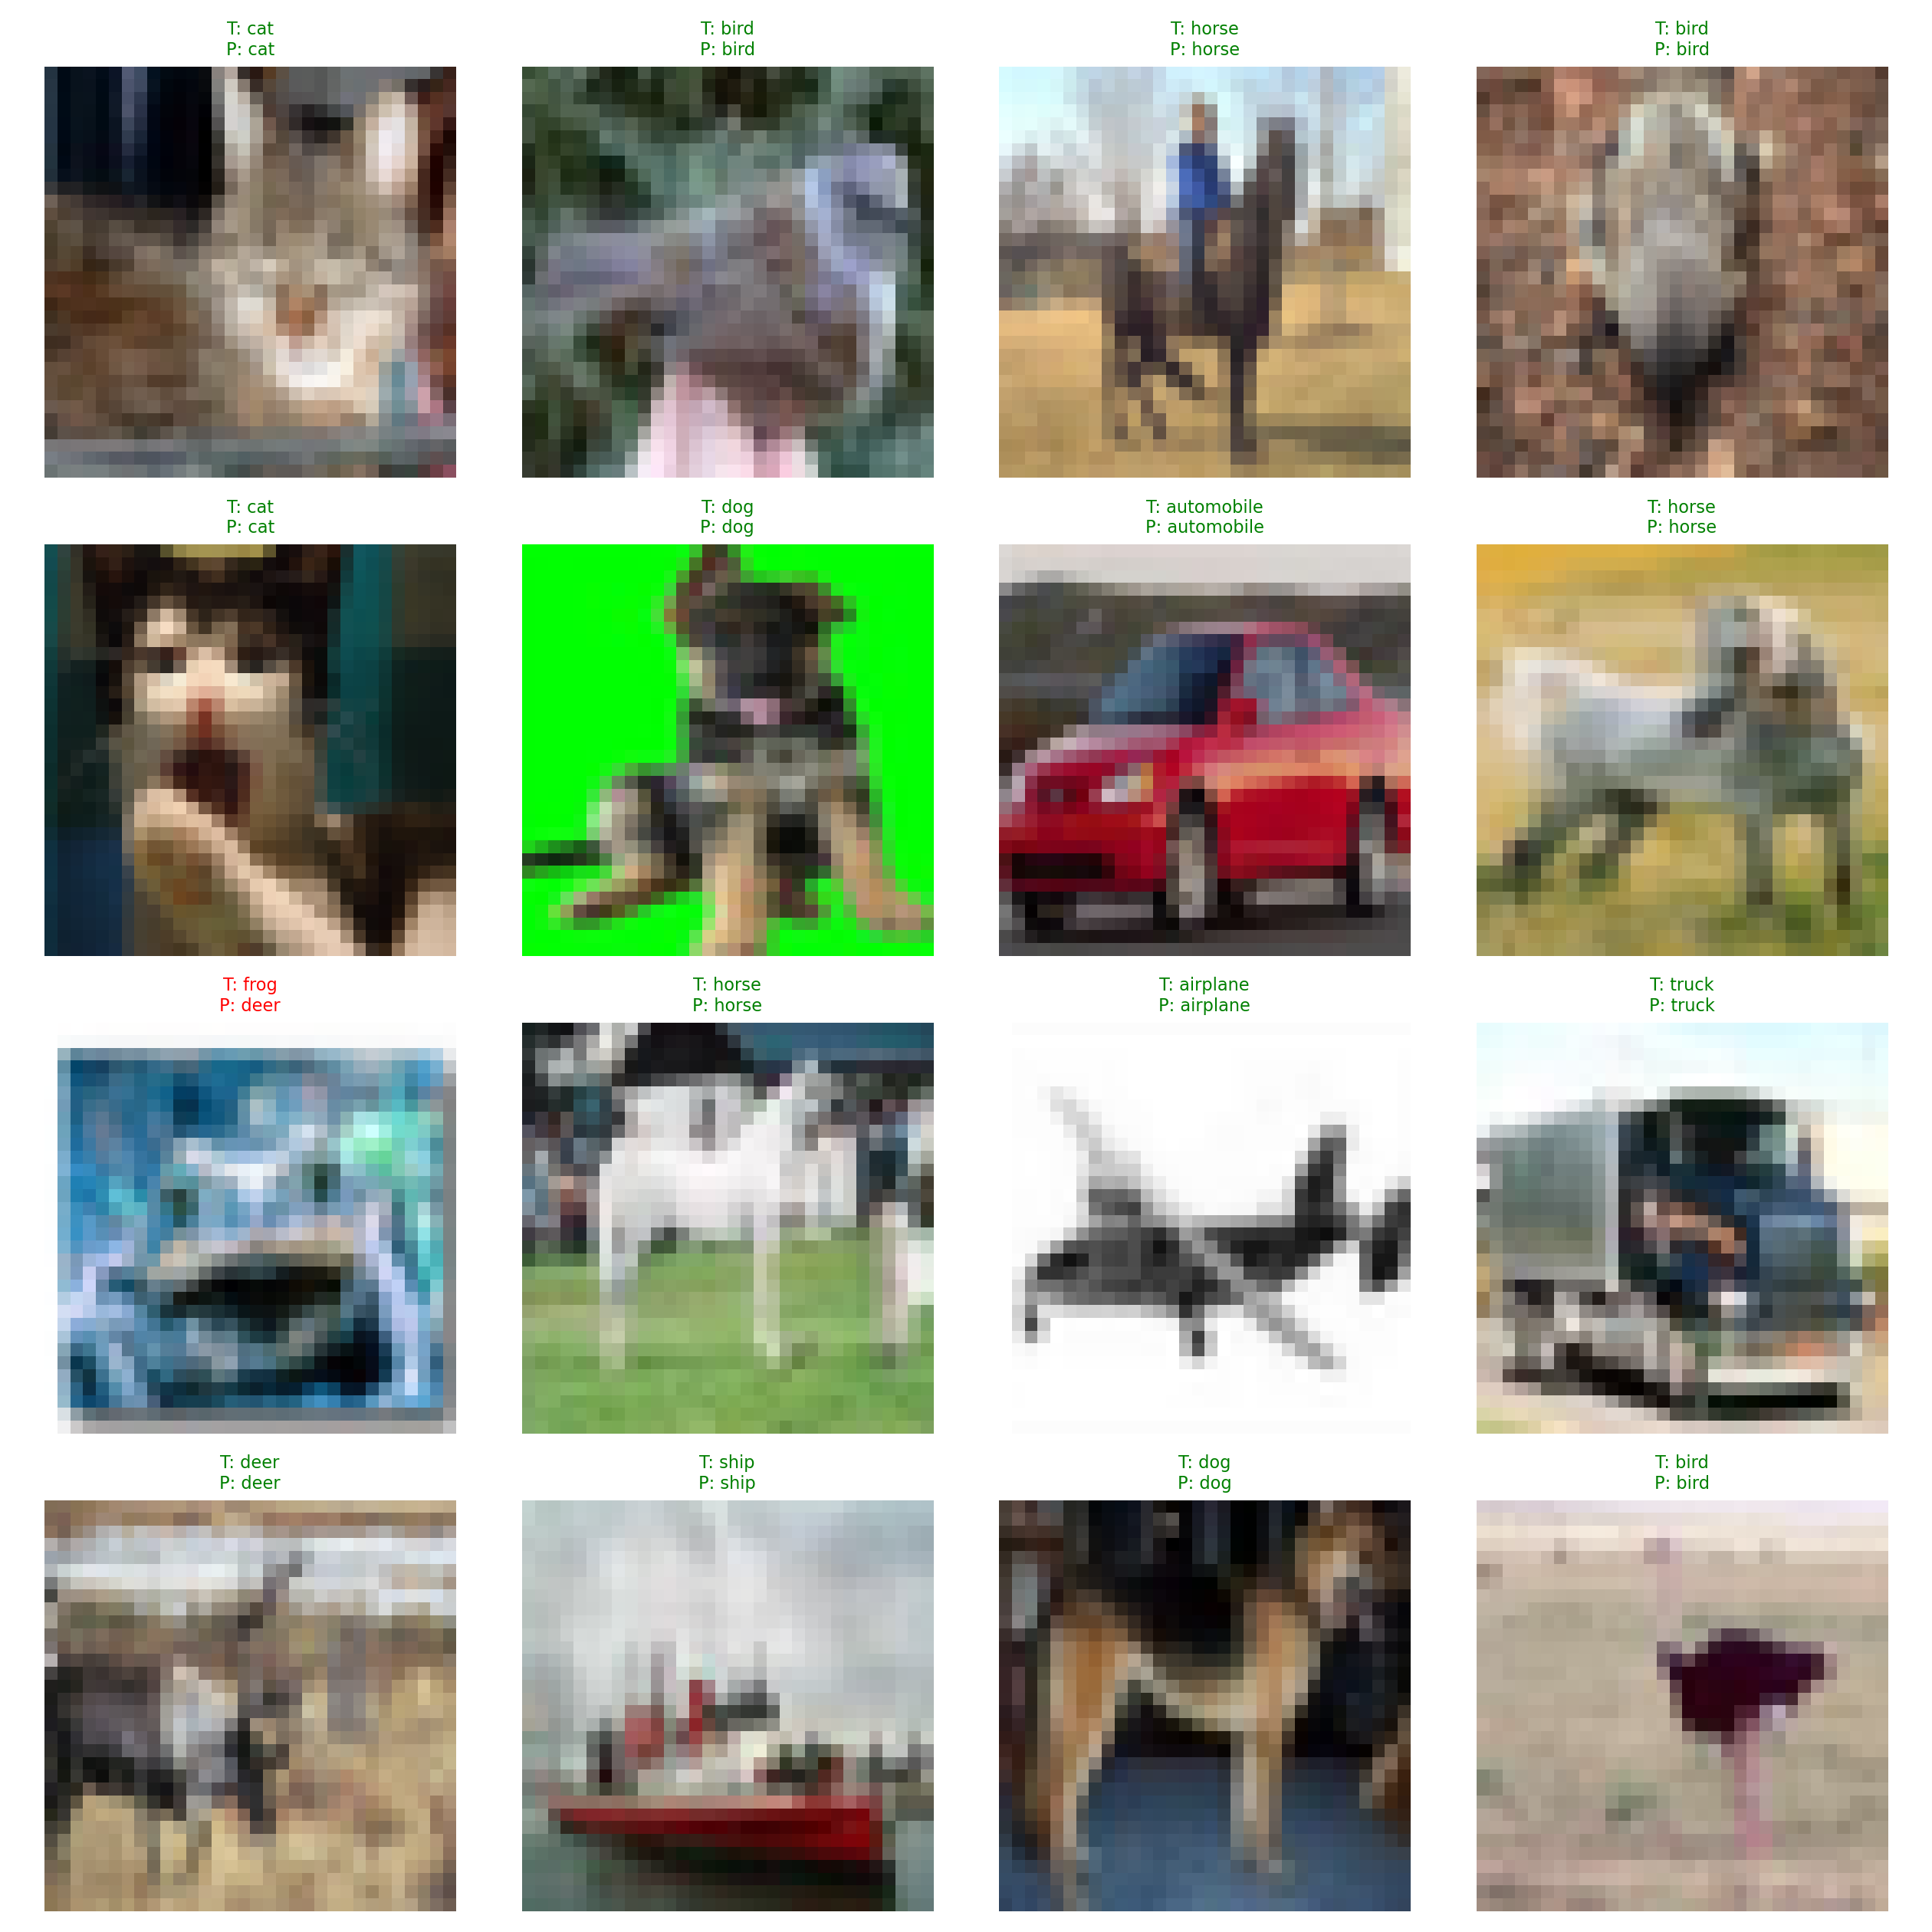
\includegraphics[width=0.85\textwidth]{../../outputs/split-impact-seed-42/plots/predictions_efficientnetb0_train95_test5.png}
    \caption{Przykładowa siatka predykcji dla najlepszej konfiguracji modelu \textbf{EfficientNetB0} (wariant train95\_test5).}
    \label{fig:predictions_effnet_best}
\end{figure}

% ============================================================
% PREDYKCJE - MOBILENETV2
% ============================================================
\begin{figure}[H]
    \centering
    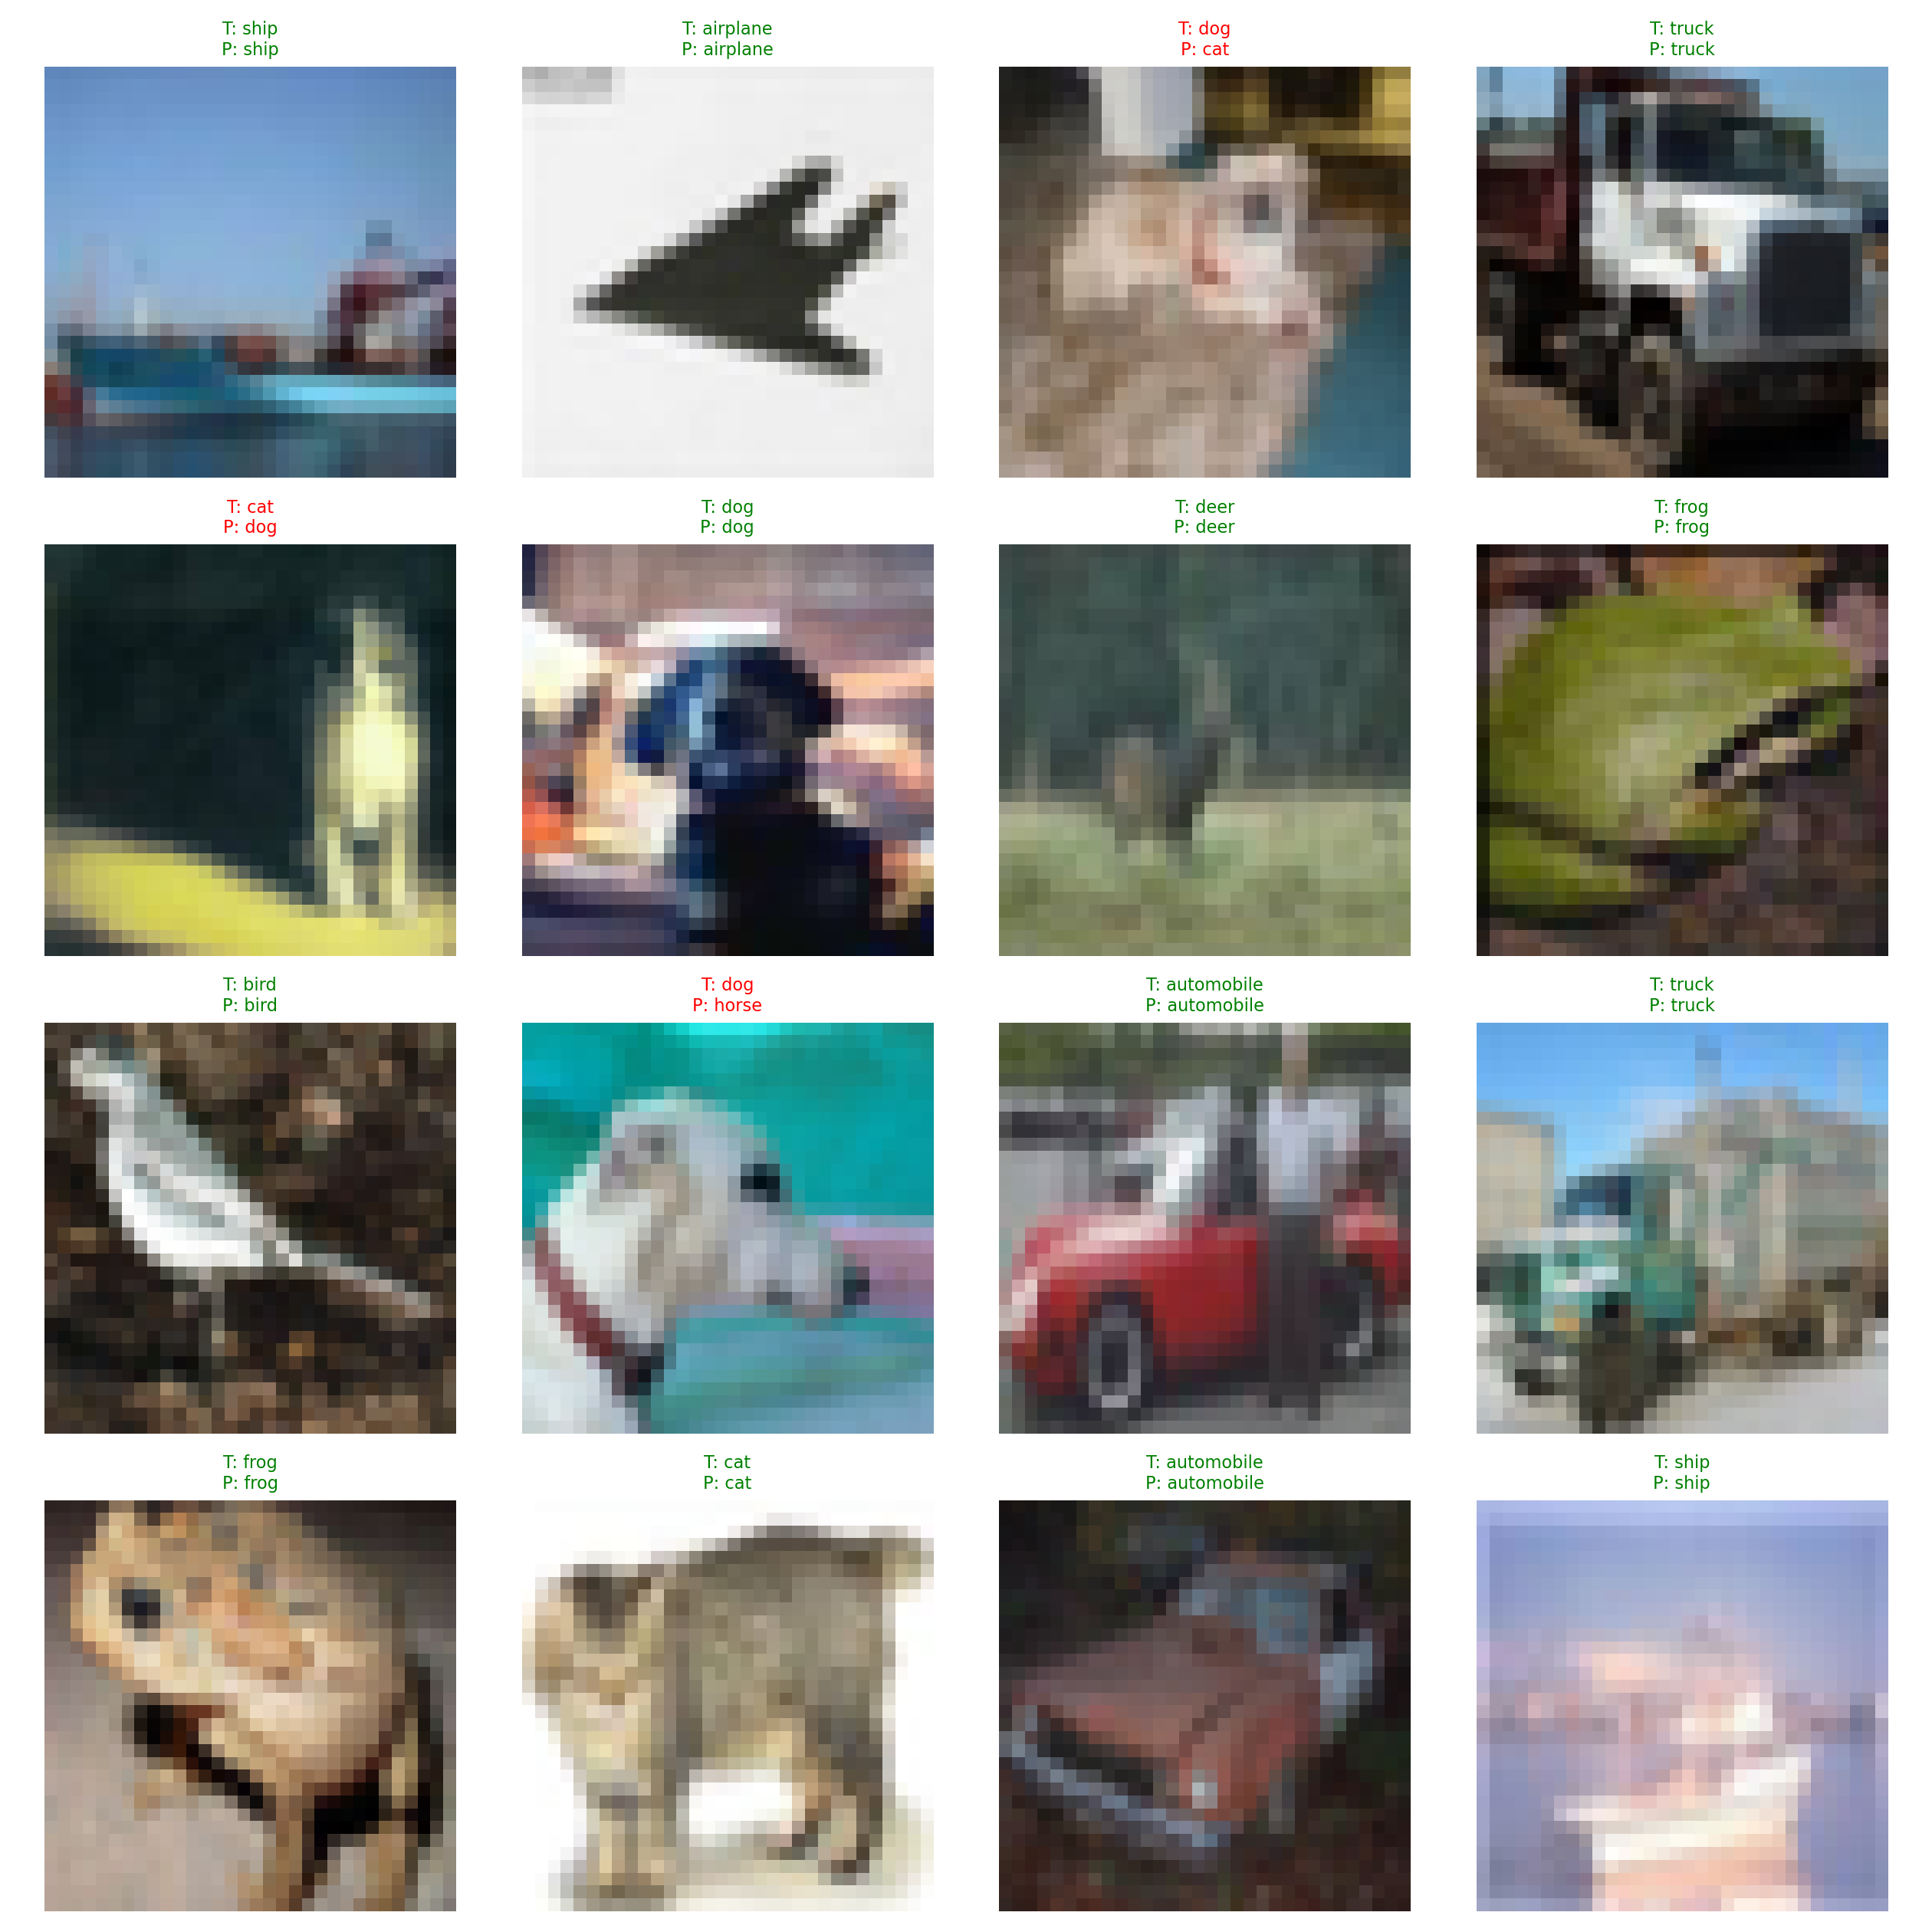
\includegraphics[width=0.85\textwidth]{../../outputs/split-impact-seed-42/plots/predictions_mobilenetv2_train90_test10.png}
    \caption{Przykładowa siatka predykcji dla najlepszej konfiguracji modelu \textbf{MobileNetV2} (wariant train90\_test10).}
    \label{fig:predictions_mobilenet_best}
\end{figure}

\section{Analiza i wnioski}

Najlepsze wyniki osiągnięto dla modelu ResNet50 przy podziale danych 90/10. Poniższa tabela przedstawia porównanie najlepszych (według miar ) osiągnięć dla każdego modelu.

\begin{table}[H]
\centering
\caption{Porównanie najlepszych wyników modeli (Peak Performance)}
\label{tab:results}
\begin{tabular}{@{}lcccr@{}}
\toprule
Model           & F1 (przy 5/95) & Peak F1 & Split Peak & Mean F1 \\ \midrule
ResNet50        & 0.8423         & 0.8993  & 0.90       & 0.8816  \\
EfficientNetB0  & 0.7802         & 0.8636  & 0.95       & 0.8396  \\
MobileNetV2     & 0.7786         & 0.8547  & 0.90       & 0.8341  \\ \bottomrule
\end{tabular}
\end{table}

\subsection{Wpływ podziału danych}
Zauważono wyraźną korelację między ilością danych treningowych a jakością modelu. Wszystkie modele wykazują szybki wzrost metryk do punktu 80/20, po którym następuje faza plateau.
\begin{itemize}
    \item Przewaga ResNet50 nad pozostałymi modelami jest najbardziej widoczna przy małych zbiorach treningowych (+0.06 F1).
    \item Przy dużych zbiorach (95/5) różnice maleją do ok. +0.02 F1.
\end{itemize}

\begin{figure}[H]
    \centering
    %\includegraphics[width=0.8\textwidth]{placeholder_learning_curve.png}
    \framebox[0.8\textwidth]{\vbox{\vspace{3cm} \centering [WYKRES: F1-Score vs Train Ratio dla 3 modeli] \vspace{3cm}}}
    \caption{Zależność miary F1 od proporcji zbioru treningowego.}
\end{figure}

\subsection{Analiza krzywych ROC}
Modele uzyskały bardzo wysokie wartości AUC (0.975 -- 0.995), co świadczy o doskonałej zdolności separacji klas. 

\begin{figure}[H]
    \centering
    \begin{minipage}{0.45\textwidth}
        \centering
        %
\includegraphics[width=\textwidth]{roc_resnet50_train5_test95.png}
        \framebox[\textwidth]{\vbox{\vspace{2cm} \centering ROC ResNet50 (5/95) \vspace{2cm}}}
    \end{minipage}
    \hfill
    \begin{minipage}{0.45\textwidth}
        \centering
        %
\includegraphics[width=\textwidth]{roc_resnet50_train90_test10.png}
        \framebox[\textwidth]{\vbox{\vspace{2cm} \centering ROC ResNet50 (90/10) \vspace{2cm}}}
    \end{minipage}
    \caption{Porównanie krzywych ROC dla modelu ResNet50 przy skrajnych podziałach.}
\end{figure}

\section{Porównanie modeli i wnioski}

\begin{enumerate}
    \item \textbf{Globalny Zwycięzca:} Model \textbf{ResNet50} okazał się bezkonkurencyjny, osiągając najwyższe wyniki we wszystkich 9 podziałach danych (Peak $F1=0.899$).
    \item \textbf{Stabilność:} ResNet50 charakteryzuje się najniższym odchyleniem standardowym wyników, co czyni go najbardziej przewidywalnym modelem w badanym zestawie.
    \item \textbf{Zdolność separacji:} Bardzo wysokie wartości ROC AUC sugerują, że błędy modelu wynikają głównie z mylenia bardzo podobnych klas, a nie z braku nauki wzorców.
    \item \textbf{Rekomendacja praktyczna:} 
    \begin{itemize}
        \item Dla najwyższej jakości: Wybór \textbf{ResNet50 + split 90/10}.
        \item Dla bezpiecznej estymacji: Wybór \textbf{splitu 80/20}, który oferuje niemal identyczną jakość przy większym (bardziej wiarygodnym) zbiorze testowym.
    \end{itemize}
\end{enumerate}

\end{document}